\label{sec:evaluation}

\newacronym{evm}{EVM}{Ethereum Virtual Machine}

This chapter aims to thoroughly evaluate the practical feasibility of the proposed concept described in chapter~\ref{sec:ttsm}. To do so, it obeys design science guidelines and, thus, uses methodologies already available in the knowledge base of workflow execution on the blockchain~\cite{hevner2004_design_science}. This ensures better reproducibility of the presented results and allows in-depth comparison to other approaches. Two artifacts are evaluated in the following: (1) the proposed concept of a \gls{ttsm} as described in section~\ref{sec:ttsm:proposal} and (2) the instantiation of the concept in the form of the prototype described in section~\ref{sec:ttsm:prototype}. Qualitative and static analysis methodologies are applied to the former, while the latter is used for experimental analysis to show real-world utility of the proposed concept.



\section{Qualitative Analysis}
\label{sec:evaluation:qualitative_analysis}
Extracting criteria for qualitative analysis is a rather tricky task, given the heterogeneous landscape of workflow execution approaches that target the blockchain (see related work chapter~\ref{sec:related-work}). However, the most often used criteria in related literature can be categorized in flexibility and privacy or security criteria. The following list of criteria was extracted from related literature to allow comparison between different approaches. To name a few, this includes~\cite{prybila_master_thesis,runtime_verification_for_bp_utilizing_bitcoin,blockchain_for_secure_io_bp,lean_architecture_for_blockchain_based_process_execution,architecture_for_multi_chain_bp_ladleif,untrusted_bp_execution_using_blockchain}.


\subsection{Flexibility Criteria}
\label{sec:evaluation:qualitative_analysis:flexibility_criteria}
In \gls{bct}-based software, flexibility is a rare trait due to the cost associated with change on the blockchain~\cite{nakamoto2009,buterin2020}. Therefore, qualitative evaluation is performed using the upcoming flexibility criteria by creating classes ranging from low flexibility to high flexibility to put the proposed concept into perspective. Notice that higher flexibility typically comes with increased architectural complexity.

\subsubsection{Blockchain Selection}
\label{sec:evaluation:qualitative_analysis:flexibility_criteria:blockchain_selection}
For many more simple real-world scenarios, predetermining a specific blockchain to be used for the entirety of the system or particular workflow instance should be enough. However, for larger and more complex workflows, there is no singular blockchain that fulfills all necessary requirements~\cite{architecture_for_multi_chain_bp_ladleif}. Taking this into consideration, and the fact that \glspl{bct} are a rather quickly evolving sector, being able to adapt different blockchains becomes a significant point of concern for \gls{bct}-based software. Figure~\ref{fig:evaluation:qualitative_analysis:blockchain_selection_classes} shows a classification of this particular criteria.

\begin{figure}[h]
    \makebox[\textwidth][c]{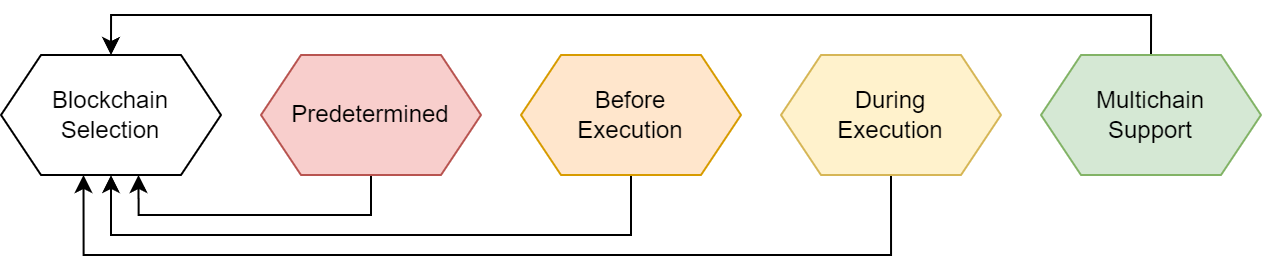
\includegraphics[width=1\textwidth]{evaluation/graphics/qualitative-analysis/blockchain-selection-classes.drawio.png}}
    \caption{A classification for blockchain selection.}
    \label{fig:evaluation:qualitative_analysis:blockchain_selection_classes}
\end{figure}

Even though there are concepts that enable multi-chain workflow execution\footnote{i.e.,\ using multiple blockchains at once that are interconnected with each other and can even exchange messages.} like the one proposed by Ladleif et al.~\cite{architecture_for_multi_chain_bp_ladleif}, most approaches rely on a single blockchain to not only execute workflows but also to tightly integrate the workflow execution system itself with the it~\cite{untrusted_bp_execution_using_blockchain,runtime_verification_for_bp_utilizing_bitcoin,bo_collaboration_between_healthcare_providers_covid_19}. The proposed concept, however, enables participants to select their preferred blockchain, and the associated desired properties, either before or dynamically during workflow execution depending on the workflow itself and the messages exchanged. This increases flexibility but also complexity due to the abstraction required.

\subsubsection{Participant Selection}
\label{sec:evaluation:qualitative_analysis:flexibility_criteria:participant_selection}
Short-running business processes and their corresponding workflows might rely on a fixed set of participants without threatening the stability or flexibility of a system or workflow. However, more volatile workflows with a considerably larger amount of participants involved need a more flexible system that enables the executing participants to select who executes certain activities on demand~\cite{fdhila2012_change_in_collaborative_processes}. Furthermore, it is advantageous for the overall workflow to select participants only after the workflow has already been launched. This allows executing participants, especially in longer-running workflows, to take environmental and political change into consideration when selecting a contractor or supplier that is required later in the workflow, for example. The classification for participant selection depicted in figure~\ref{fig:evaluation:qualitative_analysis:participant_selection_classes} differentiates between three classes ranging from least to most flexibility.

\begin{figure}[h]
    \makebox[\textwidth][c]{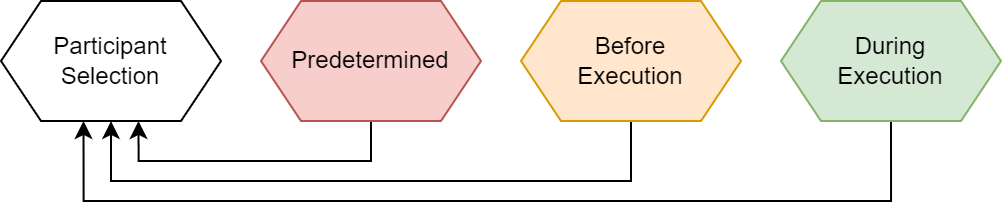
\includegraphics[width=.8\textwidth]{evaluation/graphics/qualitative-analysis/participant-selection-classes.drawio.png}}
    \caption{A classification for participant selection.}
    \label{fig:evaluation:qualitative_analysis:participant_selection_classes}
\end{figure}

Systems that predetermine all participants that are involved in the execution of workflows have not been found in related literature; however, the number of approaches that require participants to be determined before the workflow is instantiated (e.g.,\ in~\cite{modeling_blockchain_based_choreographies,inter_organizational_bps_managed_by_blockchain}), and the number of approaches that allow dynamic, or even on-demand participant selection during execution (e.g.,\ in~\cite{data_driven_choreography_data_reusability_lichtenstein,runtime_verification_for_bp_utilizing_bitcoin}), is about even. However, the concept proposed in this work does not explicitly state how participant selection should be implemented. Even though workflow definitions must specify the number of parties involved and which role they play in the overall choreography, choosing a tangible \gls{ttsm} of a participant that has been selected at a later point in time during workflow execution is still viable. This is because roles are only loosely coupled to the actual participants that carry them out. However, actions performed by participants that are no longer part of a workflow execution remain on the blockchain. This is a trait required by the persistency and verifiability properties of a \gls{ttsm} that might contradict privacy concerns to some extent\footnote{Given that no longer involved participants request data that has been associated with their participation, to be entirely removed according to the European GDPR for example.}. Nonetheless, the proposed concept technically allows any participant selection mechanism to be implemented.

\subsubsection{Workflow Mutability}
\label{sec:evaluation:qualitative_analysis:flexibility_criteria:workflow_mutability}
Being able to update workflows during execution increases flexibility even further; however, it also creates additional complexity in the form of potential issues regarding (eventual) consistency. Figure~\ref{fig:evaluation:qualitative_analysis:workflow_mutability_classes} shows a potential classification for workflow mutability.

\begin{figure}[h]
    \makebox[\textwidth][c]{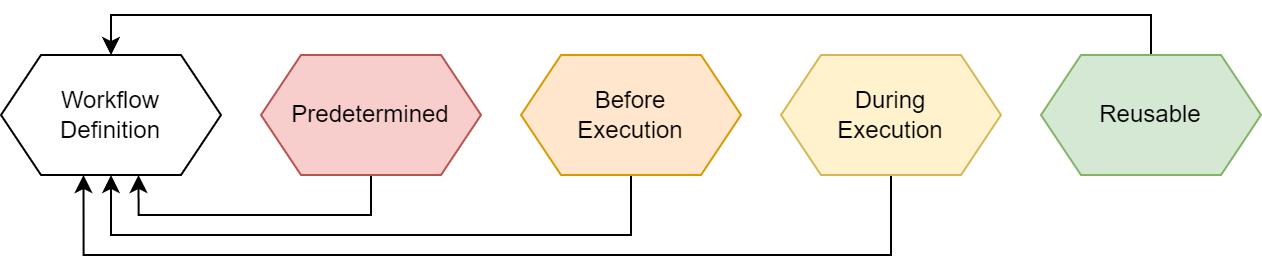
\includegraphics[width=1\textwidth]{evaluation/graphics/qualitative-analysis/workflow-mutability-classes.drawio.png}}
    \caption{A classification for workflow mutability.}
    \label{fig:evaluation:qualitative_analysis:workflow_mutability_classes}
\end{figure}

Besides predetermining workflows as part of the system being the most inflexible solution, allowing participants to define workflows themselves before execution and instantiation of the workflow itself, is the most common approach~\cite{untrusted_bp_execution_using_blockchain,bo_collaboration_between_healthcare_providers_covid_19,lean_architecture_for_blockchain_based_process_execution}. The proposed concept of this work also falls in this category performing a balancing act between complexity and reusability. Even though technically possible to adapt, allowing workflow mutability during execution or even partial reusability of already executed workflows (as described in~\cite{data_driven_choreography_data_reusability_lichtenstein}, for example) requires some changes to the concept itself. In this context, open questions like eventual consistency and participants working on different states of a workflow caused by an increased transaction inclusion duration\footnote{A commitment reference is not yet available and the command therefore not multicasted.} on certain blockchains or how to adapt reusability in \gls{bp}-centric workflow execution engines remain yet to be answered.

\subsubsection{Modelling Language}
\label{sec:evaluation:qualitative_analysis:flexibility_criteria:modelling_language}
Support for a wider range of modelling languages for workflow definitions not only improves flexibility, but also readability and reusability, because already existing process models in organizations can directly be fed into the system without the need of further adaptation. This prevents possible errors from being introduced while manually converting said models. Figure~\ref{fig:evaluation:qualitative_analysis:modelling_language_classes} includes two classifications for modelling language flexibility.

\begin{figure}[h]
    \makebox[\textwidth][c]{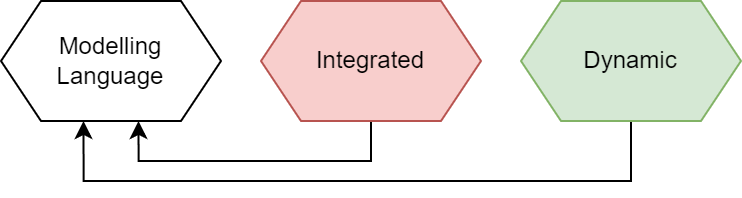
\includegraphics[width=.6\textwidth]{evaluation/graphics/qualitative-analysis/modelling-language-classes.drawio.png}}
    \caption{A classification for modelling language support.}
    \label{fig:evaluation:qualitative_analysis:modelling_language_classes}
\end{figure}

While systems, where the modelling language is tightly integrated, are strictly bound to the language semantics, dynamic approaches might require translation from one language to another. The dedicated conversion step in the workflow module (see section~\ref{sec:ttsm:proposal:from_workflow_models_to_statecharts}), puts the proposed concept on the most dynamic end of the spectrum compared to related work. Due to the internal usage of statecharts, all process models, that can be reduced to statecharts, can technically be supported. Transformations to statecharts, however, are out of scope of this work due to their complexity. Nonetheless, algorithms have been published in recent years and are publicly available for possible adaptation in a \gls{ttsm}~\cite{inter_organizational_bps_managed_by_blockchain,sequence_diagrams_to_statecharts}.


\subsection{Privacy and Security Criteria}
\label{sec:evaluation:qualitative_analysis:privacy_criteria}
Privacy is an often neglected criterion regarding workflow execution on the blockchain. In most related work, authors advise the usage of private blockchains to counteract this problem~\cite{untrusted_bp_execution_using_blockchain,bo_collaboration_between_healthcare_providers_covid_19,blockchain_based_information_sharing_in_io_workflows,lean_architecture_for_blockchain_based_process_execution,data_driven_choreography_data_reusability_lichtenstein,interpreted_bp_on_blockchain_loukil}. However, this approach only partially solves the issue, and some open problems remain. Companies might want to treat parts of internal workflows as a trade secret because they are of utmost importance to the business's success or because they are simply not relevant to the shared \gls{bp}. Another example is confidential information that is only allowed to be shared between two particular participants and must never be exposed to others\footnote{Imagine a four-party scenario where three banks and the government are involved. All participants agree on using a blockchain as a trusted third party. Some information about customers, however, is only allowed to be shared with the governmental instance and not with any other participant due to privacy regulations. Private blockchains cannot solve this issue if the privacy critical data is stored on-chain because all four participants can investigate the state of the blockchain at any point in time.}. Furthermore, the usage of private blockchains can threaten security, as previously discussed in chapter~\ref{sec:related-work}, due to the increased voting power per participant compared to public blockchains. Similar to the flexibility criteria, the upcoming privacy and security criteria are also divided into classes to put the proposed concept into perspective.

\subsubsection{Workflow Structure Sharing} \label{sec:evaluation:qualitative_analysis:privacy_criteria:workflow_structure_sharing}
Workflows that involve multiple independent participants do require sharing of workflow structures in some form to create a common frame of reference. Figure~\ref{fig:evaluation:qualitative_analysis:workflow_structure_sharing_classes} differentiates between three public and one private classification. First, public workflows that share not only their structure but also their execution context\footnote{In the form of smart contracts, for example.}. Second, public actions, where only state transitions are exposed; and third, public metadata, where only (encrypted) metadata about the workflow is shared publicly. Purely private workflows are the fourth class, in which no information is put on a blockchain that is used by more than one participant.

\begin{figure}[h]
    \makebox[\textwidth][c]{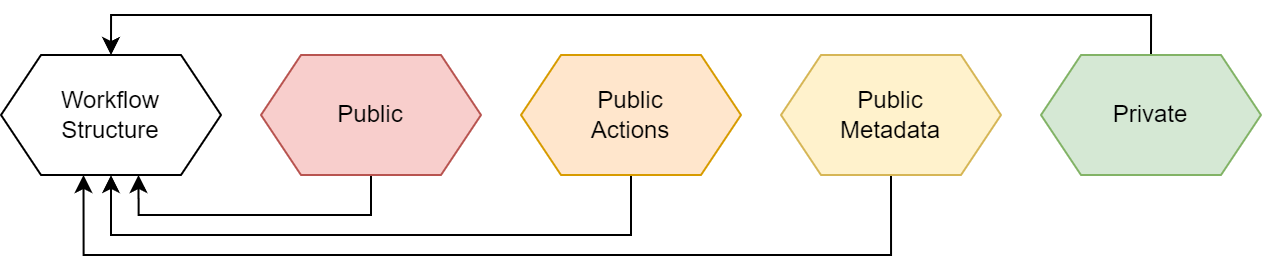
\includegraphics[width=1\textwidth]{evaluation/graphics/qualitative-analysis/workflow-structure-sharing-classes.drawio.png}}
    \caption{A classification for sharing workflow structures.}
    \label{fig:evaluation:qualitative_analysis:workflow_structure_sharing_classes}
\end{figure}

Depending on the implementation of the consistency module of a \gls{ttsm} and the chosen consistency strategy, the proposed concept might either fall into the second or third category --- sharing actions or metadata on the public blockchain, but is never executing entirely on-chain (restricted by the architecture by separating the workflow module from the consistency and persistence modules). Strategies for sharing workflow structures might include transmitting actions off-chain but storing hashes or \glspl{zkp} of actions being performed on-chain. Furthermore, the proposed concept aims to only share choreography structures that determine the required interactions between participants. Internal workflow structures can be kept entirely private or semi-private by leveraging on homomorphic encryption or \glspl{zkp}, for example.

\subsubsection{Data Sharing}
\label{sec:evaluation:qualitative_analysis:privacy_criteria:data_sharing}
The way workflow execution engines share data associated with workflows and state transitions is categorized by the classification given in figure~\ref{fig:evaluation:qualitative_analysis:data_sharing_classes}. It differentiates between data being shared over a public network and thus being available to all workflow participants, only sharing (encrypted) metadata or keeping data entirely private.

\begin{figure}[h]
    \makebox[\textwidth][c]{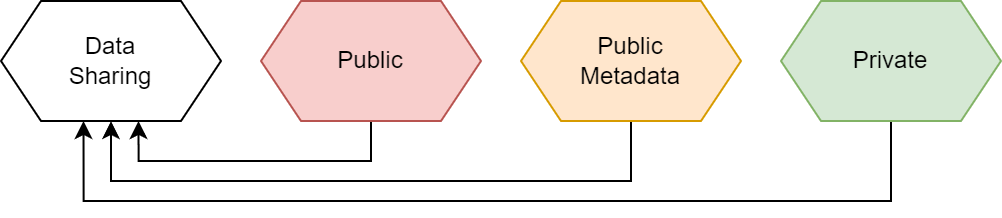
\includegraphics[width=.8\textwidth]{evaluation/graphics/qualitative-analysis/data-sharing-classes.drawio.png}}
    \caption{A classification for sharing data between participants.}
    \label{fig:evaluation:qualitative_analysis:data_sharing_classes}
\end{figure}

Most approaches found in related literature either require participants to share data entirely off-chain or entirely on-chain. The former approach neglects traceability capabilities of \glspl{bct}, and the latter restricts payload size to the maximum allowed block and transaction size of the (most often) predetermined blockchains being used. Other approaches, like the ones proposed by Lichtenstein et al.~\cite{data_driven_choreography_data_reusability_lichtenstein}, and Ladleif et al.~\cite{modeling_blockchain_based_choreographies}, which are laying their focus on the artifacts produced by workflows, also store the state and life cycle of the entire artifact on-chain and thus, makes them publicly (in the sense of ``for all participants'') available. However, the concept proposed in this work aims to bridge the gap in the related literature by only storing metadata on-chain. Similar to the workflow structures described in the previous criteria~\ref{sec:evaluation:qualitative_analysis:privacy_criteria:workflow_structure_sharing}, a \gls{ttsm} only stores hashes of actions and their associated payload data or \glspl{zkp}, for example, that ensure, that the data fulfills specific properties. Open questions, especially regarding techniques like \glspl{zkp} or homomorphic encryption, must still be solved in future work to fully leverage on the capabilities of the proposed concept.

\subsubsection{Trust}
\label{sec:evaluation:qualitative_analysis:privacy_criteria:trust}
Trust between participants is vital when they are in a conflict of interest. Studies have shown that incorporating trust as a key ingredient into workflow systems might increase workflow performance, particularly in supply chain management and logistics~\cite{fynes2005_impact_of_relationships_on_supply_chain_performance,johnston2004_supplier_trust_performance}.
A common solution to establish trust is to utilize trusted third parties~\cite{impact_of_trust_on_supply_chains,trust_in_service_oriented_ds_through_blockchain}. All approaches discussed in chapter~\ref{sec:related-work} build upon the blockchain to take up this particular role. So does the concept proposed in this work. To enable traceability through the blockchain, the consistency module of a \gls{ttsm} associates exchanged messages with commitment references. This ensures that all actions that require multi-party participation are undeniably persisted and can be verified. However, the proposed concept does not support authentication mechanisms. This means that participants occupying a particular workflow role might not be who they pretend they are. Even though workflow execution does not inflict trust-related issues, the open authentication problem might. To participate in a workflow that is handled by a \gls{bct}-based \gls{ttsm}, participants require a blockchain wallet in some form to at least provide a pseudo-identity\footnote{\glspl{bct} provide pseudo-anonymity, thus, it is practically almost impossible to authenticate a participant by her wallet information.}. However, more is needed to authenticate participants trustfully because a wallet might also belong to an attacker pretending to be a particular participant. Thus, authentication remains an open problem which is out of scope of this work due to its complexity. Future work might consider the usage of asymmetric cryptography and signatures in order to solve this issue.

\subsubsection{Conflict Resolution}
\label{sec:evaluation:qualitative_analysis:privacy_criteria:conflict_resolution}
Resolving conflicts between participants using undeniable proofs is one of the cornerstones that blockchains provide. The proposed concept leverages on this property by referencing commitments on the blockchain for each action performed by any of the participants. Therefore, conflicts can be resolved by the time-travel capabilities of a \gls{ttsm} - participants involved in a conflict can travel back in time to the point where the conflict arose. The workflow at this point in time contains all actions that led to the current state and, thus, all associated commitment references on the blockchain, which in fact, are undeniable proof of what happened\footnote{Given that the blockchain itself is tamper-proof (see consensus section~\ref{sec:background:consensus} for more details).}. Nonetheless, a follow-up issue arises regarding the authentication of participants mentioned before in criteria~\ref{sec:evaluation:qualitative_analysis:privacy_criteria:trust}. Even though a role might have performed an action according to the blockchain, this does not give proof that the action has indeed been performed by the correct participant. Due to the pseudo-anonymity of blockchains, one can not easily prove the identity of contributors without further usage of off-chain techniques such as legal contracts associating a participant to a wallet address, for example. Resolving the authentication and identity issue in future work might also solve the conflict resolution issue mentioned in this section.


\subsection{Summary and Discussion}
\label{sec:evaluation:qualitative_analysis:summary}
The qualitative analysis performed in this section has shown significant traits of the proposed concept regarding flexibility compared to existing solutions. For the most part, this can be traced back to the role of the blockchain that is only of supportive nature, a characteristic that has not been investigated in related work and \gls{bct}-based workflow execution yet. By leveraging on the blockchain without statically integrating it as a software architectural cornerstone, \glspl{ttsm} are not bound to restrictions given by the blockchain ecosystem. Compared to other concepts, this allows the concept proposed in this work to be more flexible and extensible, resulting in a highly modular architecture where components are only loosely coupled and interchangeable at any point in time. This kind of flexibility has been an unseen trait in \gls{bct}-based workflow execution engines and results in a list of advantages that are otherwise difficult to obtain, including \glspl{ttsm} switching blockchains during workflow execution without significant complexity overhead\footnote{Note that, regarding practical feasibility, participants have to determine which blockchain is best suited for which message types in order to guarantee flawless transitions during execution. Furthermore, data remains on the blockchains it was initially written to. Time travel and verification, therefore, also includes switching between blockchains.}, dynamically selecting participants on-demand, or changing the (shared or internal) workflow definition during runtime. However, two gaps in the state of the art and the proposed concept have been identified regarding blockchain interaction and authentication of participants:

\begin{itemize}
    \item Investigation of applicable techniques that store minimum amounts of data on-chain but provide maximum traceability and verifiability.
    \item Investigation of authentication techniques for blockchain participants, to prove identity (also referred to as decentralized identifiers\footnote{\url{https://w3.org/TR/did-core/} (accessed on 2022-11-29)}), to seal attack vectors like Sybil attacks.
\end{itemize}

Solving these two research problems (1) further reduces transaction cost while not endangering the traceability and verifiability that \glspl{ttsm} already provide, and (2) being able to undeniably associate actions being performed by participants with real-world identities. Nonetheless, the qualitative analysis has shown that the proposed concept combines traits from different approaches while reducing the footprint on the blockchain, preserving privacy to some extent, and improving flexibility.



\section{Static Analysis}
\label{sec:evaluation:static_analysis}
In this section, the static structure of the proposed concept is analyzed by deriving formal metrics and taking a closer look at the macro software architecture. It aims to give insight into the complexity and cost of a \gls{ttsm}. In order to do so, the remainder of this section assumes the usage of a layer-1 \gls{bct}-based consistency strategy in the consistency module to assure comparability with related work~\cite{untrusted_bp_execution_using_blockchain,interpreted_bp_on_blockchain_loukil,runtime_verification_for_bp_utilizing_bitcoin,interpreted_bp_on_blockchain_weber}. The \gls{bct}-based consistency strategy creates a peer-to-peer network where each participant is directly connected to all the other participants. An additional connection to the blockchain is established that is used to prove the integrity of each message exchanged. Other technologies, such as layer-2 rollups or using \glspl{zkp}, might yield other results.


\subsection{Network Topology}
\label{sec:evaluation:static_analysis:network_topology}
The \gls{ttsm} network topology is determined by the number of workflow participants, only including the ones that are relevant to perform a specific command. Even if the workflow requires a total of $N$ roles, certain state transitions might only interact with $n < N$ participants occupying a subset of the $N$ roles. In the following, state transitions are used exemplary for any kind of command w.l.o.g. Given a state transition that requires interaction with $n$ participants, the \textit{maximum} number of connections each participant has to establish can be derived from the fact that the \gls{ttsm} concept operates on a peer-to-peer network. Thus $n - 1$ connections must be established, excluding the participant that proposed the state transition. Therefore, the total number of connections required is equal to the number of edges in a complete graph. The computation is given in equation~\ref{eq:evaluation:static_analysis:max_number_of_connections} with $C_{max}$ being the total number of connections required. % chktex 35

\begin{equation}
\label{eq:evaluation:static_analysis:max_number_of_connections}
C_{max}(n) = \frac{n(n-1)}{2} % chktex 35
\end{equation}

The proposal of a single state transition only requires the proposing participant to connect to $n - 1$ (excluding self) involved participants. Each involved participant, excluding the proposing one, has to establish precisely one connection resulting in a total amount of $n - 1$. However, after receiving the state transition, each participant has to send an accept or reject message to all other $n - 1$ participants. Thus, resulting in a complete graph or ``fully connected mesh''. One can now derive the total number of messages exchanged $M$ when performing a state transition\footnote{Starting in the proposal phase until the transaction has been included into a block.} using equation~\ref{eq:evaluation:static_analysis:number_of_messages_per_transition}.

\begin{equation}
\label{eq:evaluation:static_analysis:number_of_messages_per_transition}
M(n) = n ^ 2 + n
\end{equation}

The number of messages per state transition is therefore quadratically bound to the number of involved participants assuming that a message is not only sent to the other $n - 1$ participants but also to one self\footnote{Imagine an exemplary scenario, where four parties are involved: (1) the product manufacturer, (2) the reseller, (3) the customs authorities and (4) the freight forwarder. When the reseller orders a product, only the reseller, and the manufacturer have to perform and accept the state transition (i.e.,\ all participants involved in an activity). Given that $N=4$ and $n=2$, the total number of messages exchanged over the network is $2^2+2=6$ and the number of connections is $\frac{2(2-1)}{2}=1$. The customs authorities and the freight forwarder may not receive any messages at all at this point.}. Expressed in Landau notation, this results in an overall communication complexity of $\mathcal{O}(n^2)$ given that $n > 1$ when performing actions w.l.o.g.


\subsection{Blockchain Transactions}
\label{sec:evaluation:static_analysis:blockchain_transactions}
Similar to the network topology, the maximum number of blockchain transactions is also determined by the number of involved participants required for a specific command. Given a total of $N$ roles and $n$ participants, launching a workflow might involve $n \geq N$ participants\footnote{A single role might be fulfilled by different participants at different points in time.}, however, performing state transitions most of the time requires $n \leq N$ participants. Thus, the maximum number of transactions on the blockchain is linear to the number of involved participants, as shown in equation~\ref{eq:evaluation:static_analysis:number_of_bc_tx_per_transition} where $TC$ is the blockchain \textit{transaction count} and $t_p$ the number of \textit{participants} involved in the command.

\begin{equation}
\label{eq:evaluation:static_analysis:number_of_bc_tx_per_transition}
TC(t) = \begin{cases}
            0 & \text{for $t_p < 1$} \\
            t_p + 1 & \text{for $t_p \geq 1$}
        \end{cases}
\end{equation}

Commands involving one participant (i.e.,\ themselves) typically do not require blockchain interaction. However, in certain scenarios, a participant might want to prove to an external party that a specific artifact existed at a particular point in time. Given that a \gls{ttsm} solely operates on statecharts, one can derive the total number of blockchain transactions per workflow instance as follows. Let $W$ be a workflow defined as statechart and formalized as 5-tuple $\langle S, s_0, F, E, T \rangle$ where S is the set of possible states, $s_0 \in S$ the initial state, $F \subseteq S$ being the set of final states and $T$ is the set of transitions. Then, the total amount of required blockchain transactions is linear to the cardinality of $T$ denoted as $|T|$ and, in case of loops or decisions in a workflow, the number of state transitions $t_c$ performed per $t \in T$ with $TC_{total}$ being the \textit{total transaction count} on the blockchain.

\begin{equation}
\label{eq:evaluation:static_analysis:total_number_of_bc_tx_per_bp}
TC_{total} = \sum_{t \in T} TC(t) \cdot t_c
\end{equation}

Equation~\ref{eq:evaluation:static_analysis:total_number_of_bc_tx_per_bp} computes the maximum number of blockchain transactions in a workflow instance as a summation of state transitions $t \in T$ and the associated number of required participants. Leveraging on the notation defined above, one can derive the average number of participants involved per state transitions $\overline{n}$ as follows.

\begin{equation}
\label{eq:evaluation:static_analysis:average_number_of_participants}
\overline{n} = \sum_{t \in T} \frac{t_p}{t_c}
\end{equation}

Given $\overline{n}$ participants that have been required to complete workflow instance $I$ on average and $m$ being the total number of state transitions performed, the overall communication complexity is linear and comes down to $\mathcal{O}(\overline{n} \cdot m)$ which simplifies to $\mathcal{O}(m)$ assuming $\overline{n}$ being the smaller factor.


\subsection{Persistence Events}
\label{sec:evaluation:static_analysis:persistence_events}
The number of persistence events dispatched by a \gls{ttsm} always has to equal or be greater than the number of blockchain transactions (see section~\ref{sec:ttsm:proposal:receiving_commands}). This is a constraint required by the persistence and verifiability properties described in section~\ref{sec:ttsm:properties} and can be formally expressed as $TC_{total} \leq EC_{total}$. To compute $EC_{total}$, one must first compute the number of persistence events per state transition. Let $T$ be the set of possible state transitions in an arbitrary statechart defined as $\langle S, s_0, F, E, T \rangle$. Then, the number of persistence events dispatched per state transition $t \in T$ is computed as follows.

\begin{equation}
\label{eq:ttsm:proposal:number_of_events_per_transition}
EC(t) = (t_p + 1) + (t_r + 1) + 1
\end{equation}

In the first step, a single participant requests a state transition. This state transition is received and persisted by all involved participants. Afterwards, the local rule system dispatches a persistence event (including the validation results) for each rule engine registered $t_r$ and one that indicates if the overall validation process was successful. In the last step, each participant has to either send an accept or reject message over the network, which results in a single persistence event per participant $t_p$. An additional event is dispatched to indicate if all involved participants accepted or at least one rejected the proposed state transition. Participants not involved in a state transition do not emit any persistence events. Therefore, the total number of persistence events $EC_{total}$ can be computed as the sum of persistence events per state transition performed.

\begin{equation}
\label{eq:ttsm:proposal:total_number_of_events_per_bp}
EC_{total} = \sum_{t \in T} EC(t) \cdot t_c
\end{equation}

One observation when comparing $EC_{total}$ to $TC_{total}$ is that $EC_{total}$ is always larger than $TC_{total}$ because, in addition to the events dispatched per participant, $EC(t)$ also includes the events dispatched by the rules module and an additional event that indicates the final status of the command.

% Similar to equation~\ref{eq:evaluation:static_analysis:total_number_of_bc_tx_per_bp}, equation~\ref{eq:ttsm:proposal:total_number_of_events_per_bp} also leverages on $t_c$ to indicate how often $t \in T$ has been performed in a workflow instance. Proving that $TC_{total} \leq EC_{total}$ holds now becomes a straightforward task by substituting for $TC_{total}$ and $EC_{total}$:

% \begin{equation}
% \sum_{t \in T} TC(t) \cdot t_c \leq \sum_{t \in T} EC(t) \cdot t_c
% \end{equation}

% It becomes clear that one is \textit{strictly larger} than the other when substituting and simplifying both functions $TC(t)$ and $EC(t)$. The lower bound $t_p \leq 1$ in $TC(t)$ is ignored because this proof is only concerned with the upper bounds of both functions:

% \begin{equation}
% \sum_{t \in T} (t_p + 1) \cdot t_c < \sum_{t \in T} (t_p + 3 + t_r) \cdot t_c
% \end{equation}

% Thus, a \gls{ttsm} always emits \textit{strictly more} persistence events than blockchain transactions required, regardless of the number of participants, resulting in $TC_{total} < EC_{total}$.

% \begin{flushright}
% $\blacksquare$
% \end{flushright}


\subsection{Summary and Discussion}
\label{sec:evaluation:static_analysis:summary}
The formal static analysis performed in this section has shown that the overall complexity of the network, required in a \gls{ttsm}, is bound quadratically to the number of participants due to the underlying ``fully connected mesh'' topology. This increases resiliency because, in theory, participants can forward messages to other participants, but it also increases the complexity of the required infrastructure. Figure~\ref{fig:evaluation:static_analysis:partially_connected_mesh} depicts a possible setup between three participants, namely Alice, Bob, and Mallory, where the direct link between Alice and Bob has been lost, and Mallory must forward messages.

\begin{figure}[h]
    \makebox[\textwidth][c]{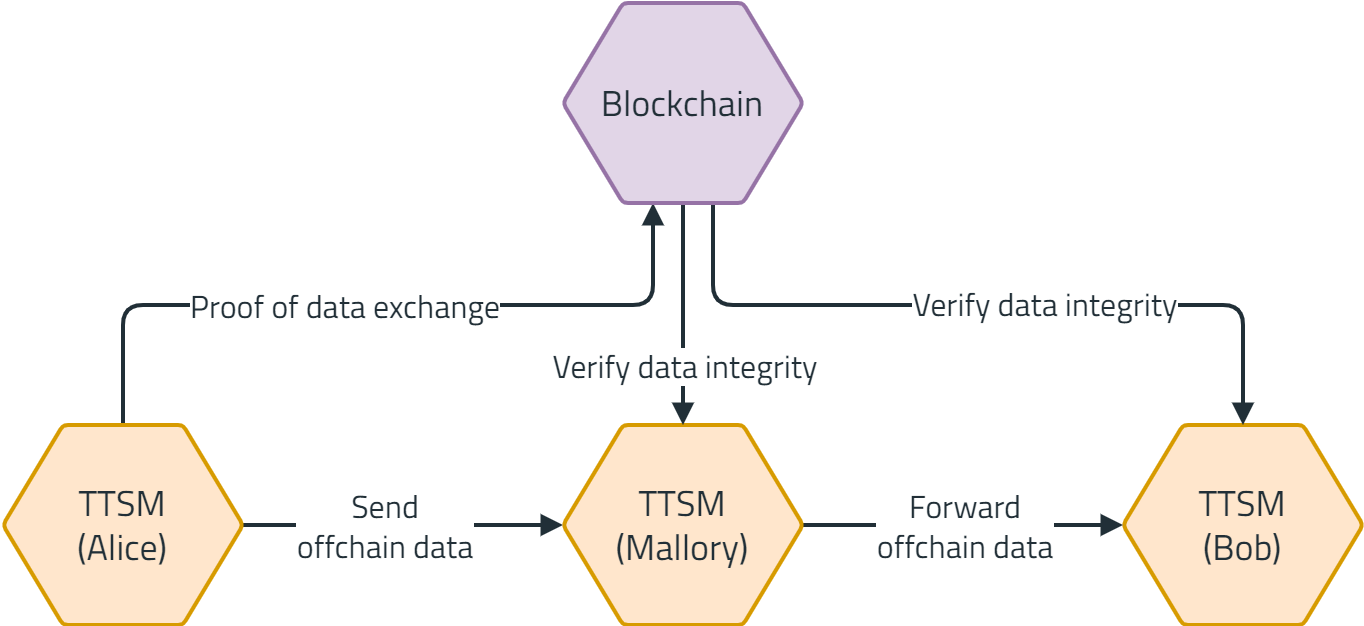
\includegraphics[width=.8\textwidth]{evaluation/graphics/static-analysis/TTSM-multiple-participants-broken-connection-2.drawio.png}}
    \caption{Mallory forwards messages from Alice to Bob.}
    \label{fig:evaluation:static_analysis:partially_connected_mesh}
\end{figure}

Setups like these are one possible mechanism supported by a \gls{ttsm} network that allows compensation of direct peer-to-peer links being lost. However, each participant must retain her connection to the blockchain to persist proof of data being exchanged and to verify the integrity of (forwarded) messages. Imagine a scenario where Alice dispatches a state transition request that Mallory must forward to Bob to complete the state transition. Instead of forwarding the original request dispatched by Alice, Mallory modifies it to make Bob accept the message and tamper with the state in a way that favors Mallory slightly and puts Bob at a disadvantage. Even though such attacks might be dangerous because they reduce the overall trust in the network, it is possible for Alice, and especially Bob, to verify the integrity of the forwarded message using the blockchain\footnote{For example, by comparing the hash of the forwarded message with the hash stored on the blockchain.}.

To better integrate compensation mechanisms into the \gls{ttsm} concept, a new consistency message that proves that a participant has indeed forwarded a message could be introduced. Two opportunities for future work have been identified:

\begin{itemize}
    \item The investigation of compensation mechanisms for lost peer-to-peer or even peer-to-blockchain connections to further increase resiliency.
    \item The investigation of algorithms with a small on-chain footprint that allow participants to verify message integrity.
\end{itemize}

Furthermore, this section has shown that the number of blockchain transactions required is linear to the number of participants involved in a particular state transition and that the number of persistence events dispatched internally by a \gls{ttsm} is strictly larger. Internal persistence events are not only dispatched for each blockchain transaction (associated with a commitment reference), but they can also be used for everything that happens only on the side of a single participant that is irrelevant for other participants. This enables a \gls{ttsm} to give participants a much finer granularity on traceability without polluting the blockchain.



\section{Scenario Simulations}
\label{sec:evaluation:simulations}
The aim of this section is to show the real-world utility of the approach proposed in this work. Different use cases are therefore simulated to conduct an experimental analysis of the concept and its prototypical implementation. Furthermore, with a strong focus on execution cost and latency, the results are compared with approaches from related work. The primary sources, used as baseline references for the upcoming evaluation, include the approaches proposed by Prybila et al.~\cite{runtime_verification_for_bp_utilizing_bitcoin}, who conducted a thorough evaluation of the execution duration of their approach, Weber et al.~\cite{untrusted_bp_execution_using_blockchain} who gave an overview of the execution cost and latency when applying their concept to a supply chain and incident management use case, and Loukil et al.~\cite{interpreted_bp_on_blockchain_loukil} who evaluated their approach against two compiled and two interpreted concepts from related literature regarding execution cost.


\subsection{Prototype Adaptations}
\label{sec:evaluation:simulations:adaptations}
Even though the high flexibility of the proposed concept, as shown in section~\ref{sec:evaluation:qualitative_analysis:flexibility_criteria}, would allow the usage of an arbitrary blockchain or layer-2 rollup, an \gls{evm}-based approach is used to improve comparability with existing approaches from related literature. Using the \gls{evm} furthermore allows Solidity byte code to be converted and ported to other blockchains and rollups such as zkSync\footnote{\url{https://zksync.io/} (accessed on 2022-11-25)} or Optimism\footnote{\url{https://optimism.io/} (accessed on 2022-11-25)} as well. The \gls{evm} consistency strategy implemented for this evaluation creates a fully connected peer-to-peer mesh network where each participant directly communicates with all the other participants. In addition, each participant establishes a connection to the \gls{evm} to store the SHA-256 hash of the exchanged message on-chain. The smart contract developed and deployed for this purpose is shown in code listing~\ref{lst:evaluation:simulations:hash_storage}.\\

\begin{lstlisting}[language=Solidity,caption=Implementation of a smart contract that stores message hashes,captionpos=b,label=lst:evaluation:simulations:hash_storage]
pragma solidity >=0.7.0 <0.9.0;

/**
 * @title Hash Storage
 * @dev Store 256-bit hash values as event log
 */
contract HashStorage {

    /**
     * @dev Stores all hashes in an event log. Using events reduces gas cost dramatically.
     */
    event StoreHash(bytes32 hash);

    /**
     * @dev Stores the given hash values as event log.
     */
    function store(bytes32 hash) public {
        emit StoreHash(hash);
    }
}
\end{lstlisting}

This very simplistic smart contract only allows the storage of 256-bit values, which is exactly the amount of data an SHA-256 hash requires. To further reduce cost, the hashes are stored as event logs only. This enables traceability but omits the need for expensive $G_{sset}$ operations with a gas cost of $20000$, only leaving a $G_{transaction}$ operation as the single most expensive operation with $21000$ gas in this smart contact. With $G_{log}$ and $G_{logtopic}$ requiring $375$ gas, and $G_{logdata}$ only requiring $8$ gas per byte stored, each hash persisted on the \gls{evm} requires less than $23000$ gas~\cite{ethereum_yellow_paper}. The integrity of an exchanged message can then be verified by fetching the transaction receipt and testing if the hash stored on the \gls{evm} is the same as the hash of the message's payload. This process is part of the \gls{evm} strategy and is depicted in code listing~\ref{lst:evaluation:simulations:verifying_received_messages}.\\ % chktex 35

\begin{lstlisting}[language=JavaScript,caption=Implementation of the verification process of messages received,captionpos=b,label=lst:evaluation:simulations:verifying_received_messages]
async receiveConsistencyMessage<T>(msg: ConsistencyMessage<T>) {

  // Retrieve transaction receipt to check if log contains correct message hash.
  const txHash = msg.commitmentReference.transactionHash;
  const tx = await Web3.eth.getTransactionReceipt(txHash);

  // Reject the message if the expected and the actual hash of the message payload differ.
  const expectedHash = tx.logs[0].data;
  const actualHash = sha256(JSON.stringify(msg.payload));
  if (expectedHash !== actualHash) {
    return 'INVALID_HASH';
  }

  // Pass the message on to other modules.
  actions$.next(msg);
  return 'OK';
}
\end{lstlisting}

If the hash differs from what has been stored on the \gls{evm}, the message is entirely omitted because its integrity cannot be verified. For reproducibility reasons, the simulations rely entirely on the \gls{evm} strategy described above. The prototypical implementation used for this evaluation is available GitHub\footnote{\url{https://github.com/danielkleebinder/ttsm-prototype} (accessed on 2022-11-29)}. The upcoming sections introduce the use cases the prototype is evaluated against, derive corresponding \gls{bpmn} diagrams, and afterwards discuss the results of the simulation runs and compare them to results from related literature.


\subsection{Scenario Descriptions}
\label{sec:evaluation:simulations:descriptions}
Three distinct scenarios have been chosen for the evaluation of the proposed concept. The first one simulates a simplified facility maintenance use case that has been created throughout the course of this work by conducting interviews with domain experts - introduced in section~\ref{sec:background:bpm:bpmn}, this scenario aims to show real-world utility of the proposed concept. The second scenario simulates a supply chain, and the third a software incident management use case as described and adapted by Weber et al.~\cite{untrusted_bp_execution_using_blockchain}, López-Pintado et al.~\cite{interpreted_bp_on_blockchain_weber}, and Loukil et al.~\cite{interpreted_bp_on_blockchain_loukil} to improve comparability and reproducibility of the results. The second and third scenarios are only briefly outlined and not further discussed.

\subsubsection{Facility Management}
\label{sec:evaluation:simulations:descriptions:fm}
The facility maintenance use case, as already partially introduced in section~\ref{sec:background:bpm:bpmn}, has been derived from interviews conducted with real-world domain experts. It describes a scenario where a building administrator has been notified\footnote{Either through a timely trigger or thorough inspection conducted by a third party, for example.} that maintenance on a facility inside the building\footnote{This might be an elevator, a vending machine, or an escalator, for example} is due. The building administrator now contacts an external maintenance contractor and prepares the facility for further inspections and the maintenance itself\footnote{By closing off the facility site, for example.}. Afterwards, the contractor starts performing the maintenance, orders spare parts if repairs are required, and sends the building administrator a notice that maintenance has been completed. After the administrator's successful inspection of the facility, the maintenance contractor sends an invoice and a maintenance report. The \gls{bpmn} diagram of this scenario is depicted in figure~\ref{fig:evaluation:simulations:maintenance_full}.

\begin{figure}[h]
    \makebox[\textwidth][c]{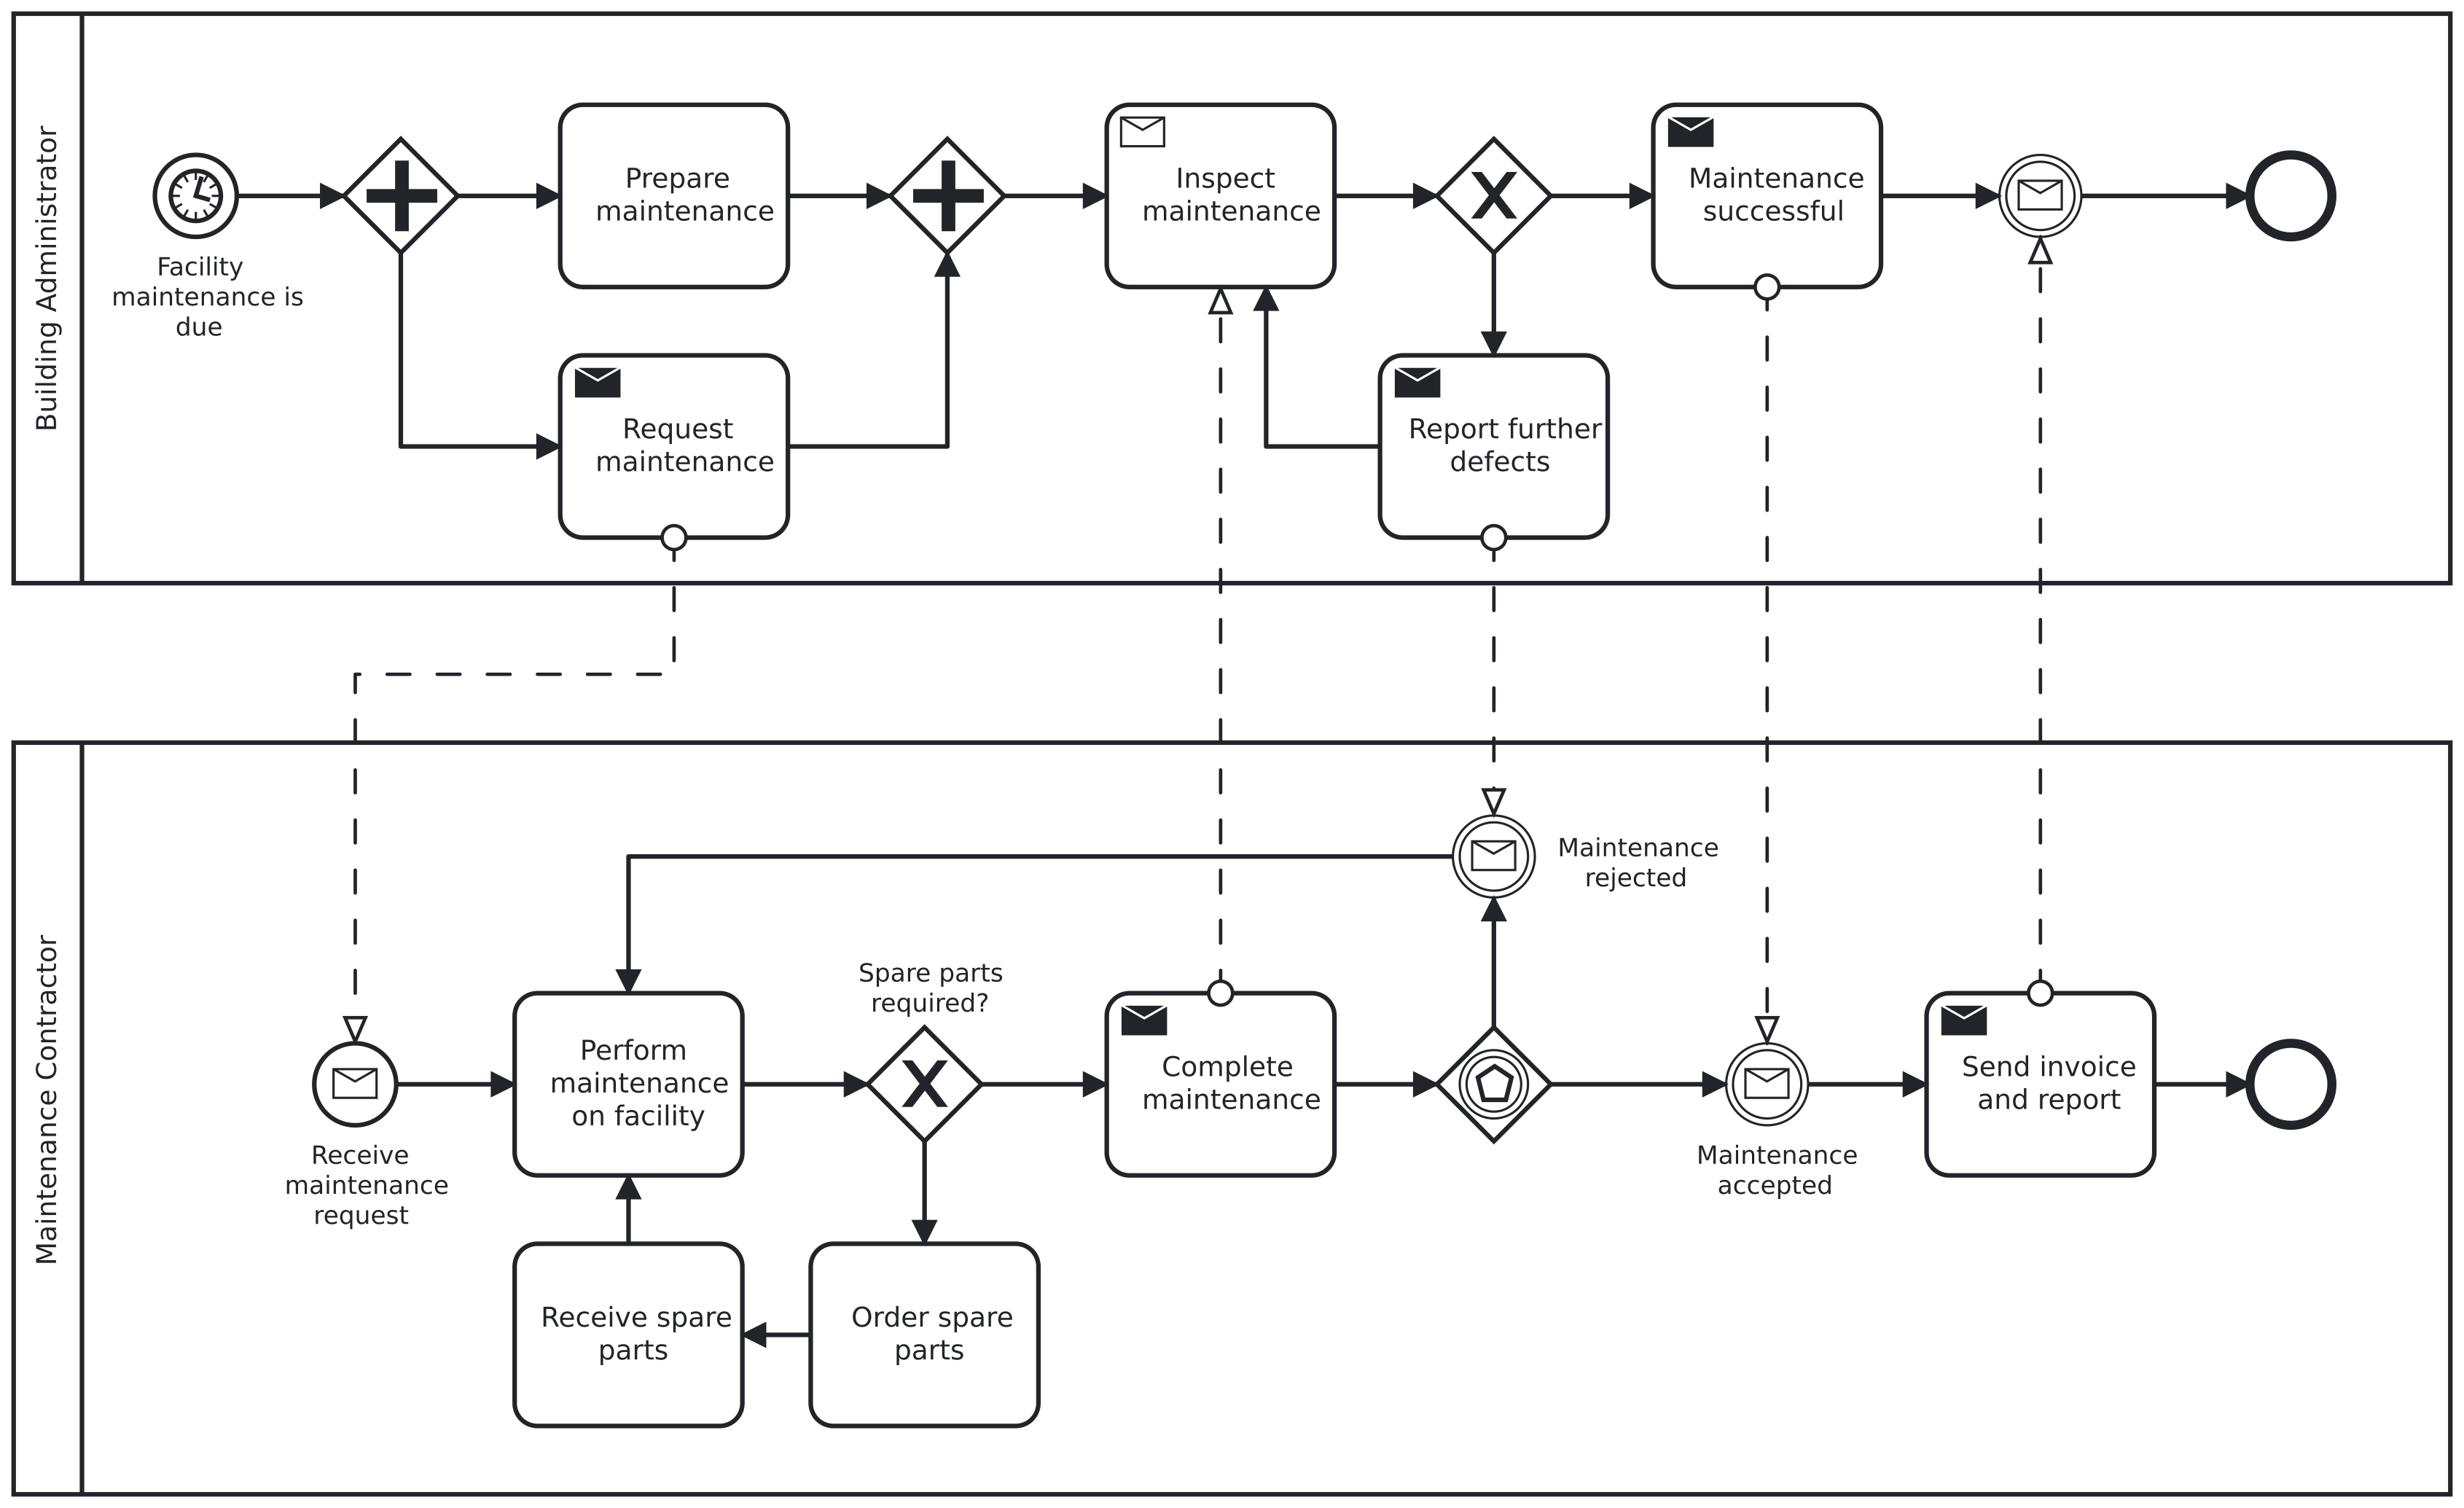
\includegraphics[width=\textwidth]{background/graphics/maintenance-full.png}}
    \caption{BPMN diagram of the facility maintenance use case introduced in~\ref{sec:background:bpm:bpmn}.}
    \label{fig:evaluation:simulations:maintenance_full}
\end{figure}

This use case should demonstrate the real-world utility of the proposed \gls{ttsm} approach. It has been simplified to some extent to use it as a stepping stone towards more complex scenarios. However, it illustrates the use of parallel and exclusive gates and the exchange of messages between participants. Therefore, the facility management scenario is an excellent first scenario to show that the proposed concept would indeed be functional in real-world environments.

\subsubsection{Supply Chain}
\label{sec:evaluation:simulations:descriptions:sc}
The supply chain use case is commonly used in related work to demonstrate the utility of a new approach and to compare its cost with other approaches. First introduced by Fdhila et al.~\cite{fdhila2015_change_in_collaborative_bps}, Weber et al.\ adapted and simplified this scenario in their work~\cite{untrusted_bp_execution_using_blockchain}. It consists of five participants interacting with each other. A bulk buyer orders a product from a manufacturer. The manufacturer then calculates what supplies in the form of raw materials and basic resources are required to produce this product and orders them from a middleman. The middleman forwards the order for the required supplies, and a carrier transports them from the supplier to the manufacturer. The manufacturer then produces the requested product and delivers it to the bulk buyer.

\begin{figure}[h]
    \makebox[\textwidth][c]{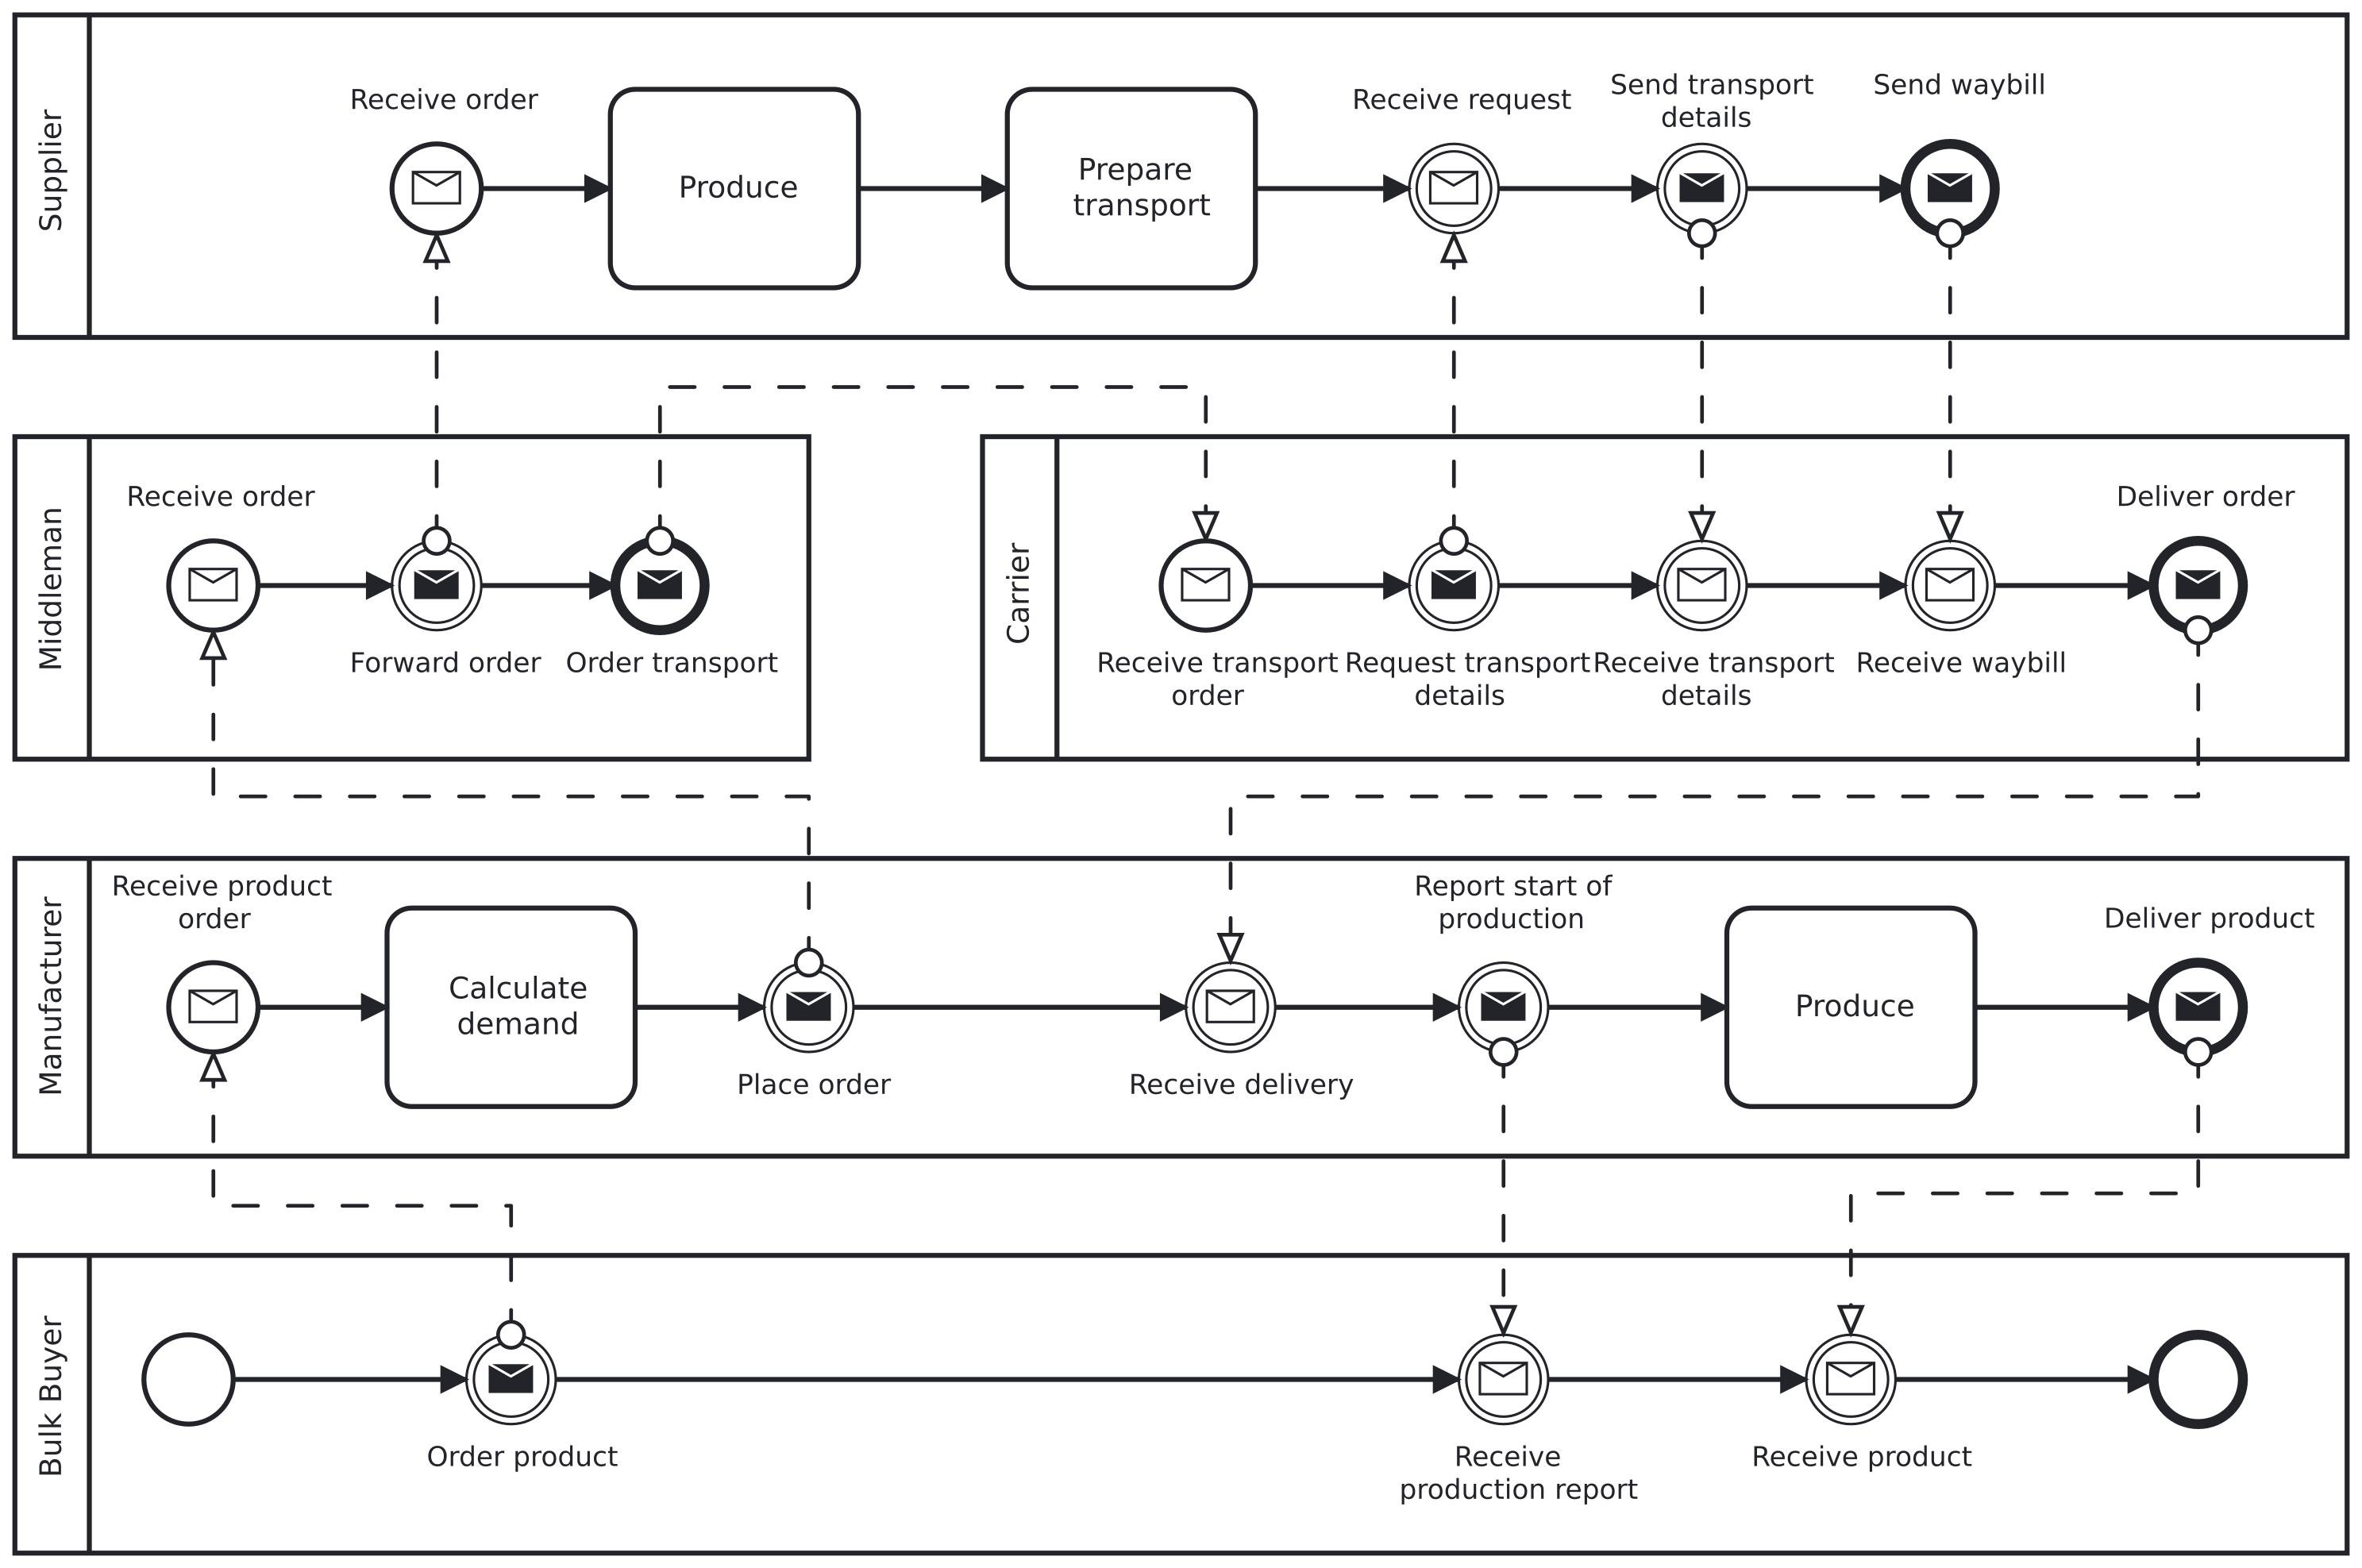
\includegraphics[width=\textwidth]{evaluation/graphics/experimental-analysis/supply-chain.png}}
    \caption{BPMN diagram of a supply chain adapted from Weber et al.~\cite{untrusted_bp_execution_using_blockchain}.}
    \label{fig:evaluation:simulations:supply_chain_full}
\end{figure}

One might realize that this supply chain has much conflict potential. Imagine the bulk buyer ordering a product that must arrive before a deadline. If the deadline is not met by the manufacturer, she has to pay penalties. To be on time, the manufacturer orders supplies through the middleman. However, the requested supplies arrived three days later than expected and were not in the correct quantity. This puts the manufacturer, whose time frame now has shifted, in a tough spot and the carrier since the manufacturer might refuse to accept the incomplete delivery. Therefore, the supply chain scenario can be used quite well to demonstrate conflict resolution capabilities~\cite{untrusted_bp_execution_using_blockchain,interpreted_bp_on_blockchain_loukil}.

\subsubsection{Incident Management}
\label{sec:evaluation:simulations:descriptions:im}
The incident management use case is, similar to the supply chain use case, a commonly encountered scenario in related work. First discussed in ``BPMN 2.0 by Example''~\cite{omg2010_bpmn_by_example}, it found its way into the domain of workflow execution on the blockchain through Weber et al.~\cite{untrusted_bp_execution_using_blockchain} and was then further adapted by many more authors in the sense of design science for comparability reasons~\cite{optimized_execution_of_bp_using_petri_nets_on_blockchain,interpreted_bp_on_blockchain_weber,lean_architecture_for_blockchain_based_process_execution,interpreted_bp_on_blockchain_loukil}.

\begin{figure}[h]
    \makebox[\textwidth][c]{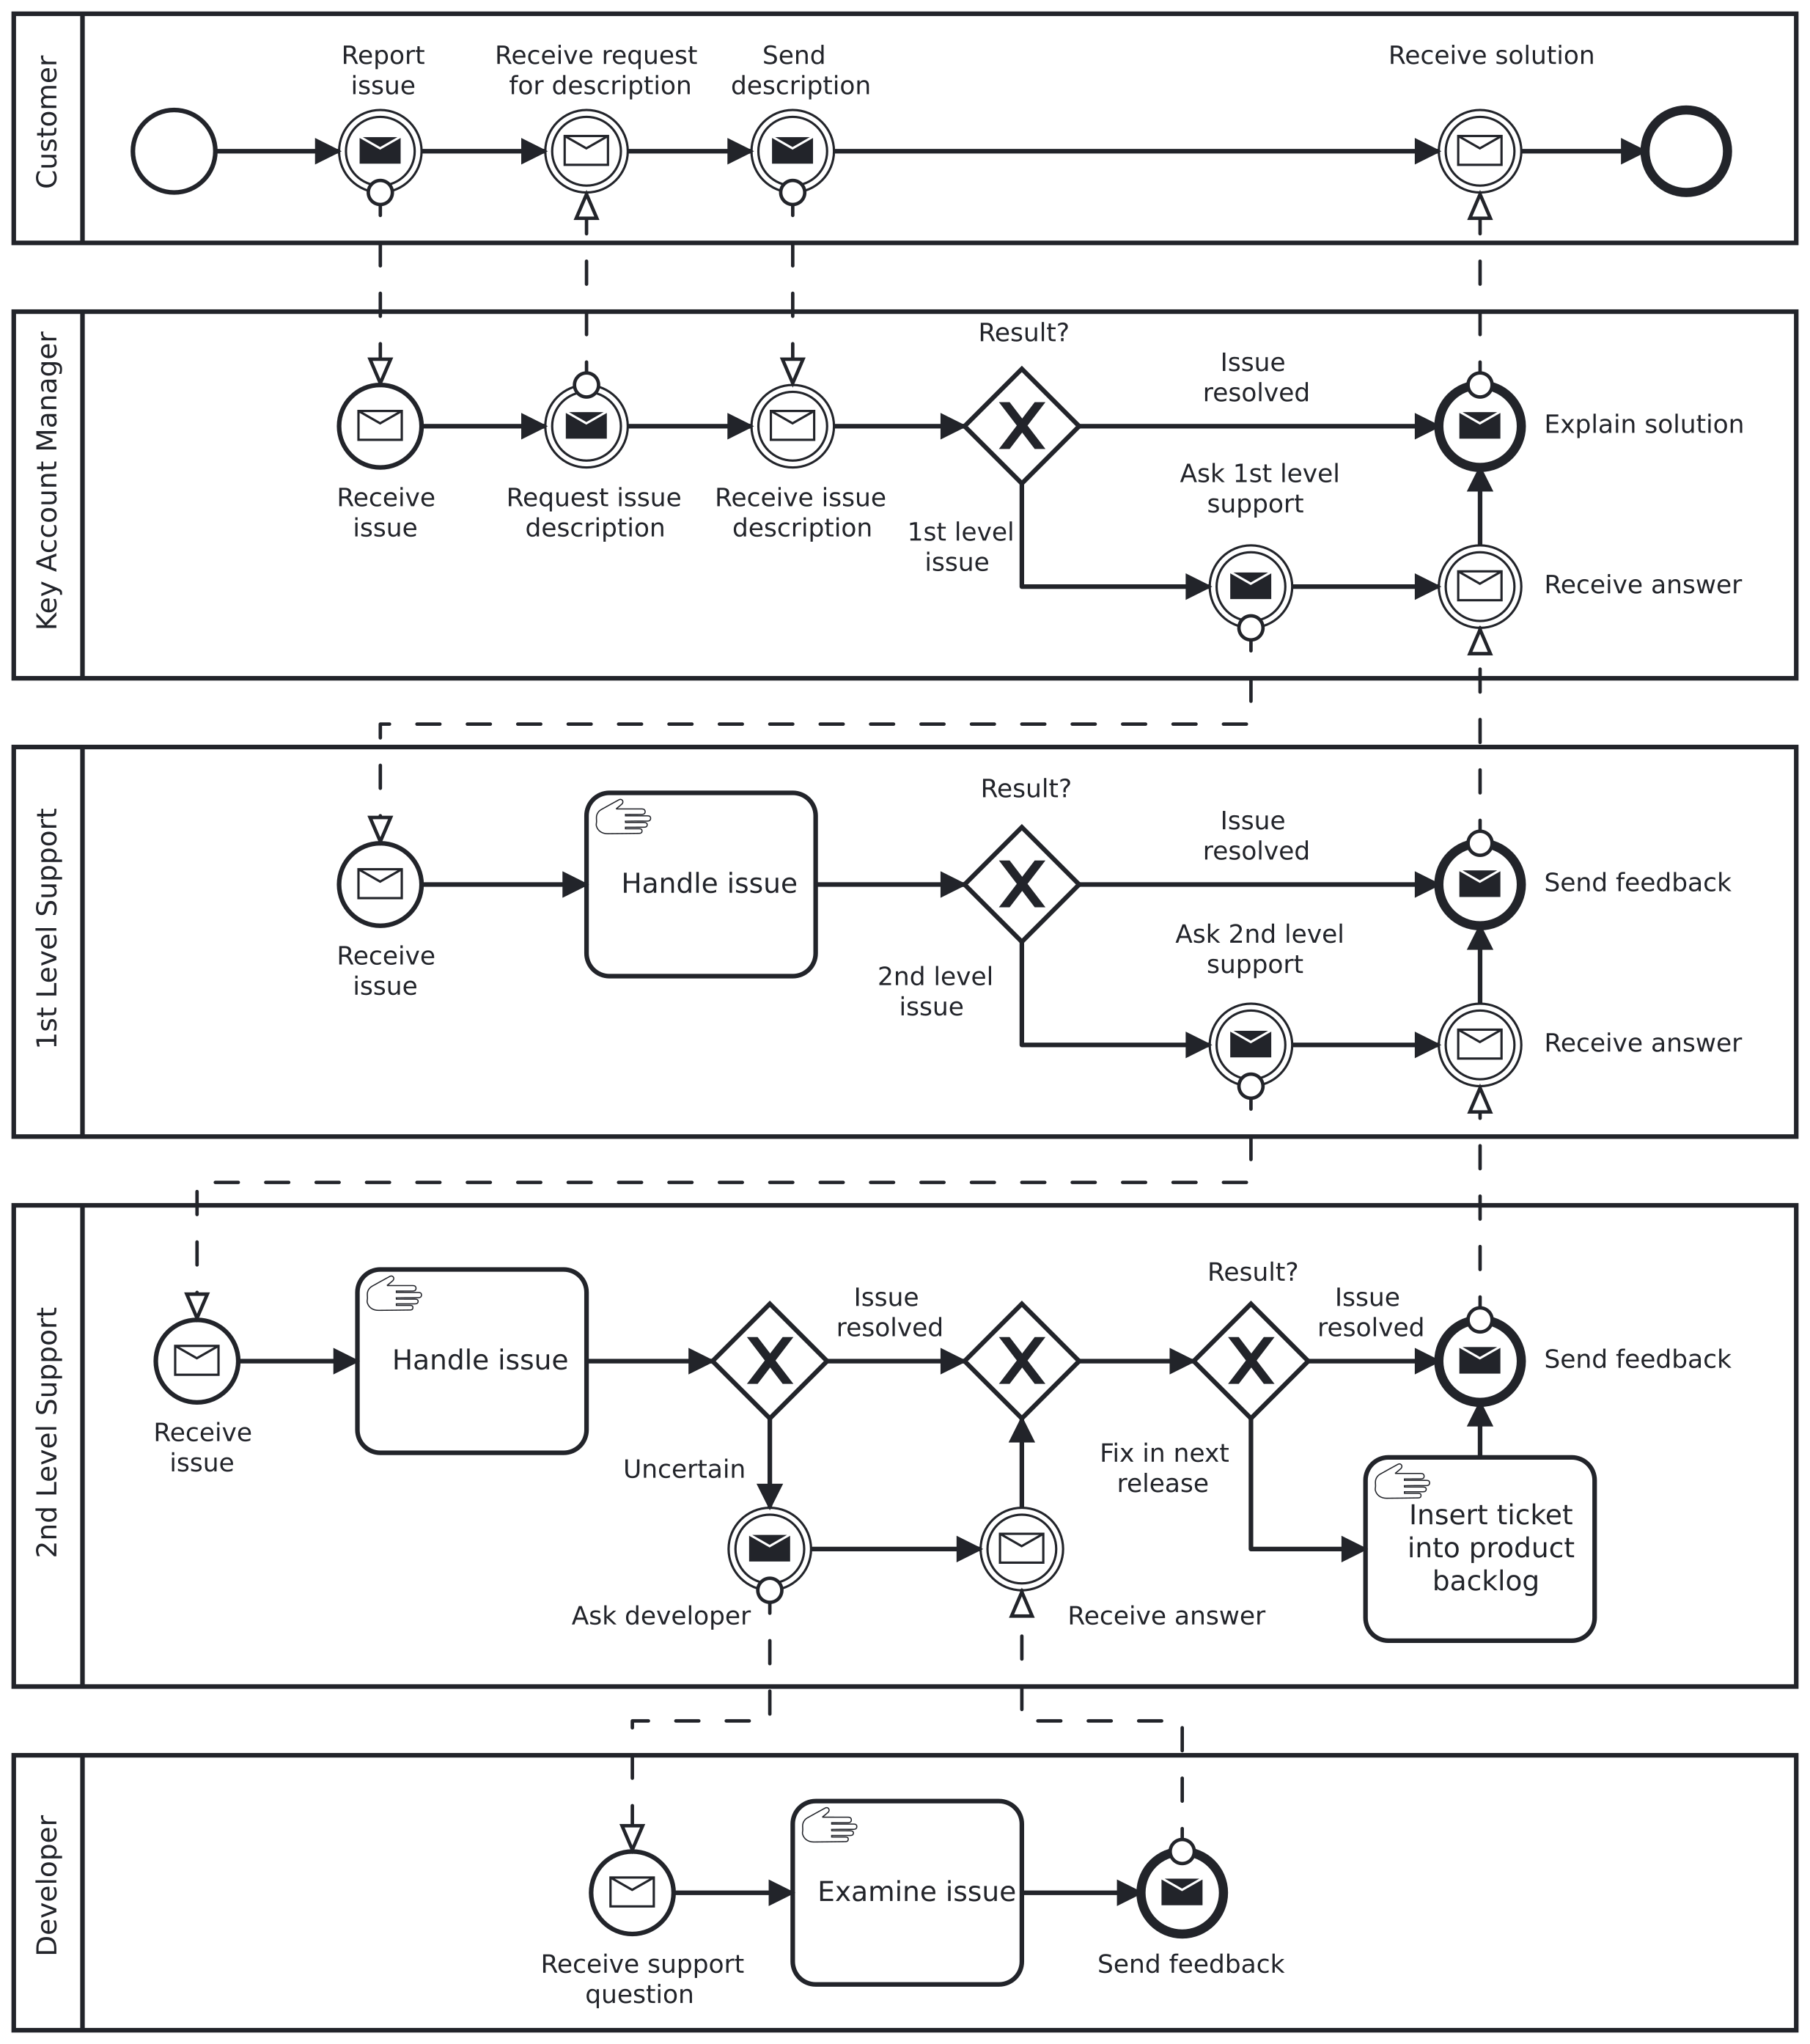
\includegraphics[width=.8\textwidth]{evaluation/graphics/experimental-analysis/incident-management.png}}
    \caption{BPMN diagram of the incident management use case adapted from ``BPMN 2.0 by Example''~\cite{omg2010_bpmn_by_example}.}
    \label{fig:evaluation:simulations:incident_management_full}
\end{figure}

Figure~\ref{fig:evaluation:simulations:incident_management_full} depicts the \gls{bpmn} diagram of the entire incident management use case. It follows an issue reported by a customer who noticed a problem with a particular software component. The issue then goes through multiple support layers, starting with the key account manager. If the key account manager cannot solve the issue by herself, she hands it over to the 1\textsuperscript{st} level support. If the 1\textsuperscript{st} level support cannot resolve the issue, it is passed on to the 2\textsuperscript{nd} level support who either asks a software developer for assistance or immediately creates a ticket and puts it into the products backlog. This relatively sophisticated business process includes more gateways and a strict separation of participants\footnote{Developers can only talk to 2\textsuperscript{nd} level support, 2\textsuperscript{nd} level support can only talk to developers and 1\textsuperscript{st} level support and so on.}.


\subsection{Discussion of Results}
\label{sec:evaluation:simulations:summary}
The evaluation results in the upcoming sections have been obtained by extracting only the communication between participants as choreography diagrams. The choreography diagram for the facility management scenario is depicted in figure~\ref{fig:background:maintenance_full_choreography}. For the supply chain and incident management scenarios, the same choreography diagrams have been used as in the related literature. These diagrams are both depicted in the work of Loukil et al.~\cite{interpreted_bp_on_blockchain_loukil}. Afterwards, semantically equivalent statecharts have been derived using the Stately editor\footnote{\url{https://stately.ai/} (accessed on 2022-10-10)} and fed into the \gls{ttsm} prototype. Finally, a script was employed to automate the process of deploying, instantiating, and executing the scenarios to ensure that each sample is executed with comparable constraints and conditions. Table~\ref{tab:evaluation:simulations:structural_comparison} gives a brief overview of the structure of each scenario.

\begin{table}[h]
\centering
\begin{tabular}{|l|r|r|r|}
    \hline
    \textbf{Scenario} & \textbf{Participants} & \textbf{Tasks} & \textbf{Gateways} \\
    \hline
    Facility Maintenance & 2 & 5 & 1 \\
    Supply Chain & 5 & 10 & 2 \\
    Incident Management & 5 & 9 & 6 \\
    \hline
\end{tabular}
\caption{Structural comparison of the choreography diagrams and statecharts of the evaluated scenarios}
\label{tab:evaluation:simulations:structural_comparison}
\end{table}

The supply chain and incident management scenarios used in this work have the same structural properties as those used for evaluation in related literature~\cite{untrusted_bp_execution_using_blockchain,optimized_execution_of_bp_using_petri_nets_on_blockchain,interpreted_bp_on_blockchain_weber,lean_architecture_for_blockchain_based_process_execution,interpreted_bp_on_blockchain_loukil}. This not only improves comparability but also reproducibility of the results. The evaluation itself is also fully automated and can be triggered after setting up the prototype project and specifying an applicable consistency strategy.

\subsubsection{Confirmation Correctness}
\label{sec:evaluation:simulations:confirmation_correctness}
The capabilities of detecting incorrect workflow traces have been evaluated according to the methodologies defined by Weber et al.~\cite{untrusted_bp_execution_using_blockchain} and Loukil et al.~\cite{interpreted_bp_on_blockchain_loukil}. A workflow trace is a path from one task in a workflow instance to another final task. For the evaluation, 500 traces have been randomly generated by shuffling a predefined set of all state transitions $T$ of a given workflow $W$ to generate a new set of distinct traces $D$, where $D$ has a cardinality of 500. Furthermore, $\forall T' \in D: T' = T$, however, $T'$ has a unique permutation of elements in $D$. This results in two subsets $D_{c} \subseteq D$ and $D_{n} \subseteq D$, where $D_{c}$ is the set of conforming traces\footnote{Traces that can be used in a given workflow.} and $D_{n}$ the set of non-conforming traces\footnote{Traces that cannot be used in a given workflow.} such that $D_{c} \cap D_{n} = \emptyset$. All traces have been correctly identified by the \gls{ttsm} prototype according to their correctness. A list of the results per scenario can be found in table~\ref{tab:evaluation:simulations:confirmation_correctness}.

\begin{table}[h]
\centering
\begin{tabular}{|l|r|c|c|}
    \hline
    \textbf{Scenario} & \textbf{Type} & \textbf{Samples} & \textbf{Correctness} \\
    \hline
    Facility Maintenance & Conforming     & 206 & 100\% \\
                         & Non-Conforming & 294 & 100\% \\
    Supply Chain         & Conforming     & 180 & 100\% \\
                         & Non-Conforming & 320 & 100\% \\
    Incident Management  & Conforming     & 197 & 100\% \\
                         & Non-Conforming & 303 & 100\% \\
    \hline
\end{tabular}
\caption{Average execution duration of each scenario}
\label{tab:evaluation:simulations:confirmation_correctness}
\end{table}

The results show that the proposed concept performs equally as well as existing solutions regarding the identification of correct and incorrect traces~\cite{untrusted_bp_execution_using_blockchain,interpreted_bp_on_blockchain_loukil}. Nonetheless, the \gls{ttsm} prototype has shown better resiliency and a higher tolerance for conforming traces because it can recover when an invalid state transition event has been dispatched. This is caused by the underlying XState library that ignores invalid state transitions and preserves the current state. Overall, the results presented in this section are in line with expectations.

\subsubsection{Blockchain imposed Latency}
\label{sec:evaluation:simulations:execution_duration}
Overall latency of the system and ensuring finality or even just inclusion of commands into blocks by a \gls{ttsm} are expected to be tightly coupled to the block time of the chosen \gls{bct}. Methodologies from related work such as Prybila et al.~\cite{runtime_verification_for_bp_utilizing_bitcoin}, and Weber et al.~\cite{untrusted_bp_execution_using_blockchain} have been employed to further investigate latency imposed by the transaction inclusion duration\footnote{Also referred to as consistency and persistence properties of a \gls{ttsm} (see section~\ref{sec:ttsm:properties}).} of the system. For the evaluation, it is assumed that all participants are available at any time.

As of section~\ref{sec:ttsm:proposal}, commands in a \gls{ttsm} are dispatched into the network of workflow participants and accepted or rejected by each of them. This is a two-step process which, if transactions are required to be included into a block of a blockchain before the \gls{ttsm} can continue, requires at least two blocks to be produced --- one in which the command is proposed and one in which participants accepted or rejected the command. The average transaction inclusion time is determined by the central limit theorem given in equation~\ref{eq:evaluation:simulations:central_limit_theorem} where $\mu$ is the overall mean of the random samples $X_1,X_2,\ldots,X_n,\ldots$, while $\bar{X}_{n}$ is the mean of the first $n$ samples and $\sigma_{\bar{X}}=\sigma/\sqrt{n}$ with $\sigma^2$ being the variance.

\begin{equation}
\label{eq:evaluation:simulations:central_limit_theorem}
Z=\lim_{n \to \infty}\left(\frac{\bar{X}_{n} - \mu}{\sigma_{\bar{X}}}\right)
\end{equation}

Given that completely finalizing a command takes at least two blocks, the median of the normal distribution is $\frac{3}{2} \cdot b_t$ where $b_t$ is the average block time. This assumption is supported by the empirical evaluation results in table~\ref{tab:evaluation:simulations:transaction_inclusion_duration} equally for all types of commands across all scenarios. Regarding the simulation itself, at the time of writing this work, there are two proof-of-stake test networks available for Ethereum in particular, namely Sepolia\footnote{\url{https://sepolia.dev/} (accessed on 2022-11-25)} and Goerli\footnote{\url{https://goerli.net/} (accessed on 2022-11-25)}. In conjunction with Alchemy\footnote{\url{https://alchemy.com/} (accessed on 2022-11-25)}, a platform that provides tooling for web3 development, Goerli was used to run the simulations. All simulations used the same smart contract which was previously deployed --- this is similar to how a \gls{ttsm} would operate on the Ethereum main network in real-world scenarios as well. Afterwards, the workflow for each use case (facility management, supply chain and incident management) were created and instantiated exactly 50 times. After successful instantiation, each workflow was executed 10 times which results in the depicted number of samples in table~\ref{tab:evaluation:simulations:transaction_inclusion_duration} below.

\begin{table}[h]
\centering
\begin{tabular}{|l|c|c|c|}
    \hline
    & \multicolumn{3}{c|}{\bfseries Facility Management} \\ \cline{2-4}
    & Samples & Av.\ Duration & Std. Dev. ($\sigma$) \\
    \hline
    Workflow Definition    & 50  & 18.209 s & 3.8 s \\
    Workflow Instantiation & 50  & 17.847 s & 3.6 s \\
    State Transition       & 50  & 17.921 s & 3.1 s \\
    \hline
    & \multicolumn{3}{c|}{\bfseries Supply Chain} \\ \cline{2-4}
    & Samples & Av.\ Duration & Std. Dev. ($\sigma$) \\
    \hline
    Workflow Definition    & 50  & 17.383 s & 3.5 s \\
    Workflow Instantiation & 50  & 18.619 s & 3.9 s \\
    State Transition       & 100 & 17.441 s & 3.5 s \\
    \hline
    & \multicolumn{3}{c|}{\bfseries Incident Management} \\ \cline{2-4}
    & Samples & Av.\ Duration & Std. Dev. ($\sigma$) \\
    \hline
    Workflow Definition    & 50  & 17.538 s & 3.4 s \\
    Workflow Instantiation & 50  & 17.112 s & 3.7 s \\
    State Transition       & 90  & 17.985 s & 3.3 s \\
    \hline
\end{tabular}
\caption{Average duration of each operation type}
\label{tab:evaluation:simulations:transaction_inclusion_duration}
\end{table}

The results were extracted from multiple test runs of the \gls{ttsm} prototype. Given that the block time of Ethereum, and in this case the Goerli test network, averages at around 12 seconds, it takes at least $\frac{3}{2} \cdot 12 = 18$ seconds to ensure that a command, including the participants responses, has been integrated into a new block on the blockchain. However, the standard deviation $\sigma$ of the samples is rather large. This distribution originates from the randomization of execution times for each command resulting in a 12 to 24 seconds execution duration. Some commands have been dispatched immediately after a new block has been mined, resulting in an overall duration of around two block times (i.e.,\ $24$ seconds), while others have been dispatched at the end of a block and thus have been integrated into said block almost immediately after dispatching, resulting in a duration of just above one block time (i.e.,\ $>12$ seconds). The execution duration distribution is depicted as box plot in figure~\ref{fig:evaluation:simulations:box_chart_transaction_inclusion}.

\begin{figure}[h]
    \makebox[\textwidth][c]{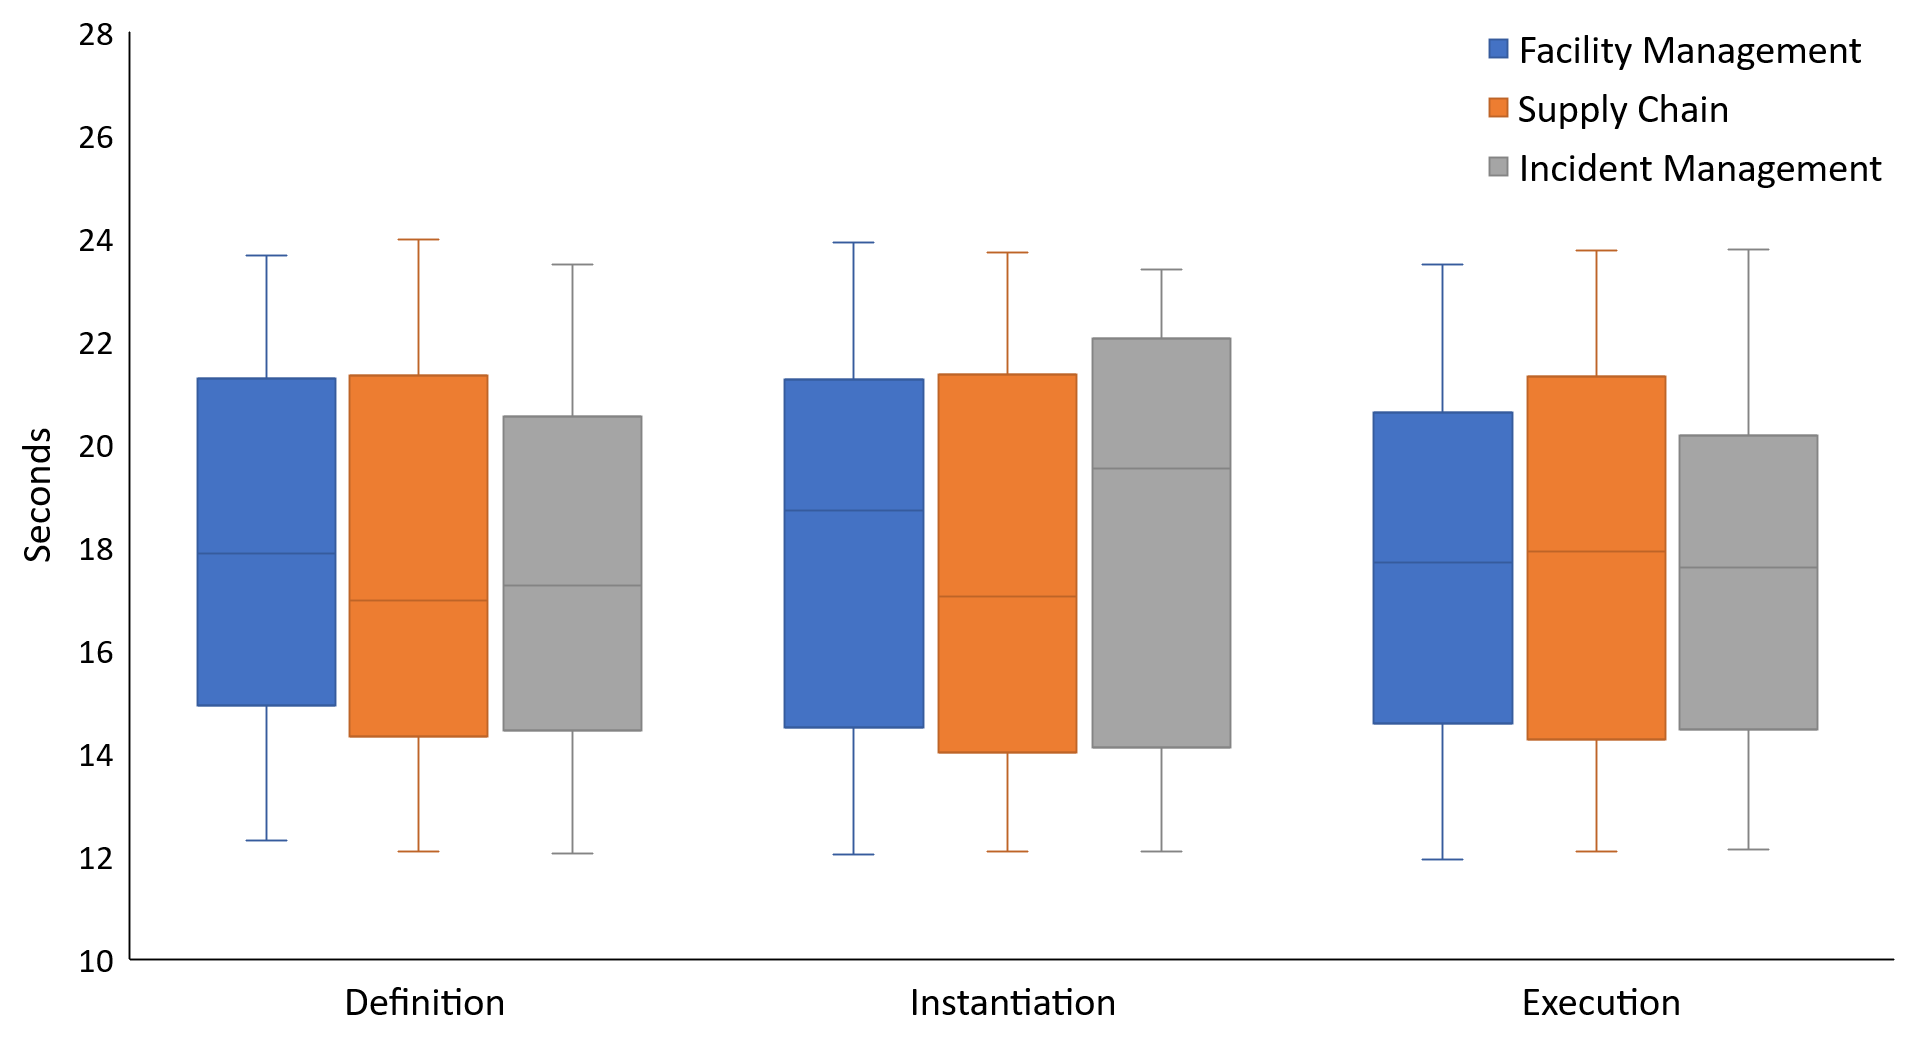
\includegraphics[width=.85\textwidth]{evaluation/graphics/experimental-analysis/enforced-finality-box-chart.png}}
    \caption{Box plot illustrating a one to two block time (12 s -- 24 s) command duration imposed by the blockchain.}
    \label{fig:evaluation:simulations:box_chart_transaction_inclusion}
\end{figure}

Nonetheless, the proposed \gls{ttsm} concept technically also supports \textit{optimistic workflow execution}. This kind of execution aims to eliminate the latency introduced by the blockchain. It enables participants to dispatch and distribute new commands to the workflow network without having to wait until the blockchain has produced a new block in which an integrity proof of the command is included. The aim of optimistic workflow execution\footnote{Later on also referred to as \textit{optimistic execution}.} is to create a system that is close to the status quo of off-chain \gls{bpm} engines regarding workflow execution duration and performance. While \textit{enforced transaction inclusion}\footnote{Later on also referred to as \textit{enforced inclusion}.} halts workflow execution while waiting for the command integrity transaction to be included in the next block\footnote{Which is required to generate a blockchain transaction receipt holding the commitment reference.}, \textit{optimistic execution} immediately sends the command to all involved participants and afterwards waits for the blockchain response.

If the participant who dispatched the optimistic command eventually receives the transaction receipt, she creates a new consistency event that associates the optimistic command with the commitment reference from the receipt. Even though \textit{optimistic execution} is much faster than \textit{enforced inclusion}, participants must expect rollbacks at a later point in time when the blockchain catches up. If the integrity transaction cannot be included in a block on the blockchain or if any of the participants notice that an outstanding optimistic command is still missing its commitment reference after a predefined period of time, the command becomes invalid. This rolls the entire workflow state back to the point in time where it was still valid. The consistency and persistence events stored are still preserved inside the event bus for traceability reasons; however, the event sourcing systems of each particular module, which require a correct and consistent state, only accumulate events until the invalid one is reached. All events received after the rollback are then, once again, treated as valid ones.

Only a superficial \textit{optimistic execution} implementation is provided in the \gls{ttsm} prototype that eliminates the latency introduced by the blockchain but does not incorporate a rollback mechanism due to its complexity. Nonetheless, all scenarios have also been executed in this superficial \textit{optimistic execution} mode. The evaluation results are given in table~\ref{tab:evaluation:simulations:optimistic_duration}.

\begin{table}[h]
\centering
\begin{tabular}{|l|c|c|c|}
    \hline
    & \multicolumn{3}{c|}{\bfseries Facility Management} \\ \cline{2-4}
    & Samples & Av.\ Duration & Std. Dev. ($\sigma$) \\
    \hline
    Workflow Definition    & 50  & 0.019 s & 0.008 s \\
    Workflow Instantiation & 50  & 0.331 s & 0.033 s \\
    State Transition       & 50  & 0.114 s & 0.055 s \\
    \hline
    & \multicolumn{3}{c|}{\bfseries Supply Chain} \\ \cline{2-4}
    & Samples & Av.\ Duration & Std. Dev. ($\sigma$) \\
    \hline
    Workflow Definition    & 50  & 0.018 s & 0.005 s \\
    Workflow Instantiation & 50  & 0.041 s & 0.019 s \\
    State Transition       & 100 & 0.079 s & 0.033 s \\
    \hline
    & \multicolumn{3}{c|}{\bfseries Incident Management} \\ \cline{2-4}
    & Samples & Av.\ Duration & Std. Dev. ($\sigma$) \\
    \hline
    Workflow Definition    & 50  & 0.019 s & 0.005 s \\
    Workflow Instantiation & 50  & 0.023 s & 0.006 s \\
    State Transition       & 90  & 0.184 s & 0.069 s \\
    \hline
\end{tabular}
\caption{Average duration of each operation type using \textit{optimistic execution}}
\label{tab:evaluation:simulations:optimistic_duration}
\end{table}

The execution duration per command has been reduced to the workflow logic and network latency itself, entirely omitting the delay imposed by the blockchain. Table~\ref{tab:evaluation:simulations:finality_vs_optimistic_total} compares the total workflow execution duration of each scenario using \textit{enforced transaction inclusion} and \textit{optimistic workflow execution} modes.

\begin{table}[h]
\centering
\begin{tabular}{|l|c|c|c|c|c|c|}
    \hline
    \multirow{2}{*}{\bfseries Scenario} &
    \multicolumn{3}{c|}{\bfseries Enforced Inclusion} &
    \multicolumn{3}{c|}{\bfseries Optimistic Execution} \\ \cline{2-7}
    & Samples & Av.\ Dur. & $\sigma$ & Samples & Av.\ Dur. & $\sigma$ \\
    \hline
    Facility Management & 10 & 57 s & 3.1 s & 10 & 0.57 s & 0.3 s  \\
    Supply Chain        & 10 & 181 s & 16.8 s & 10 & 0.79 s & 0.3 s \\
    Incident Management & 10 & 149 s & 10.3 s & 10 & 1.65 s & 0.5 s \\
    \hline
\end{tabular}
\caption{Total duration of finality enforced and optimistic workflow execution}
\label{tab:evaluation:simulations:finality_vs_optimistic_total}
\end{table}

As illustrated before, choosing one execution mode over the other has a significant impact on the overall duration. When using \textit{enforced inclusion} mode, waiting for the command integrity transaction to be included in a new block on the Ethereum blockchain imposes a noteworthy latency. Figure~\ref{fig:evaluation:simulations:pie_chart_transaction_inclusion_portion} shows a pie chart depicting the duration required for the execution of the workflow logic (including network delays) and puts it against the downtime that transaction inclusion requires when explicitly enforced.

\begin{figure}[h]
    \makebox[\textwidth][c]{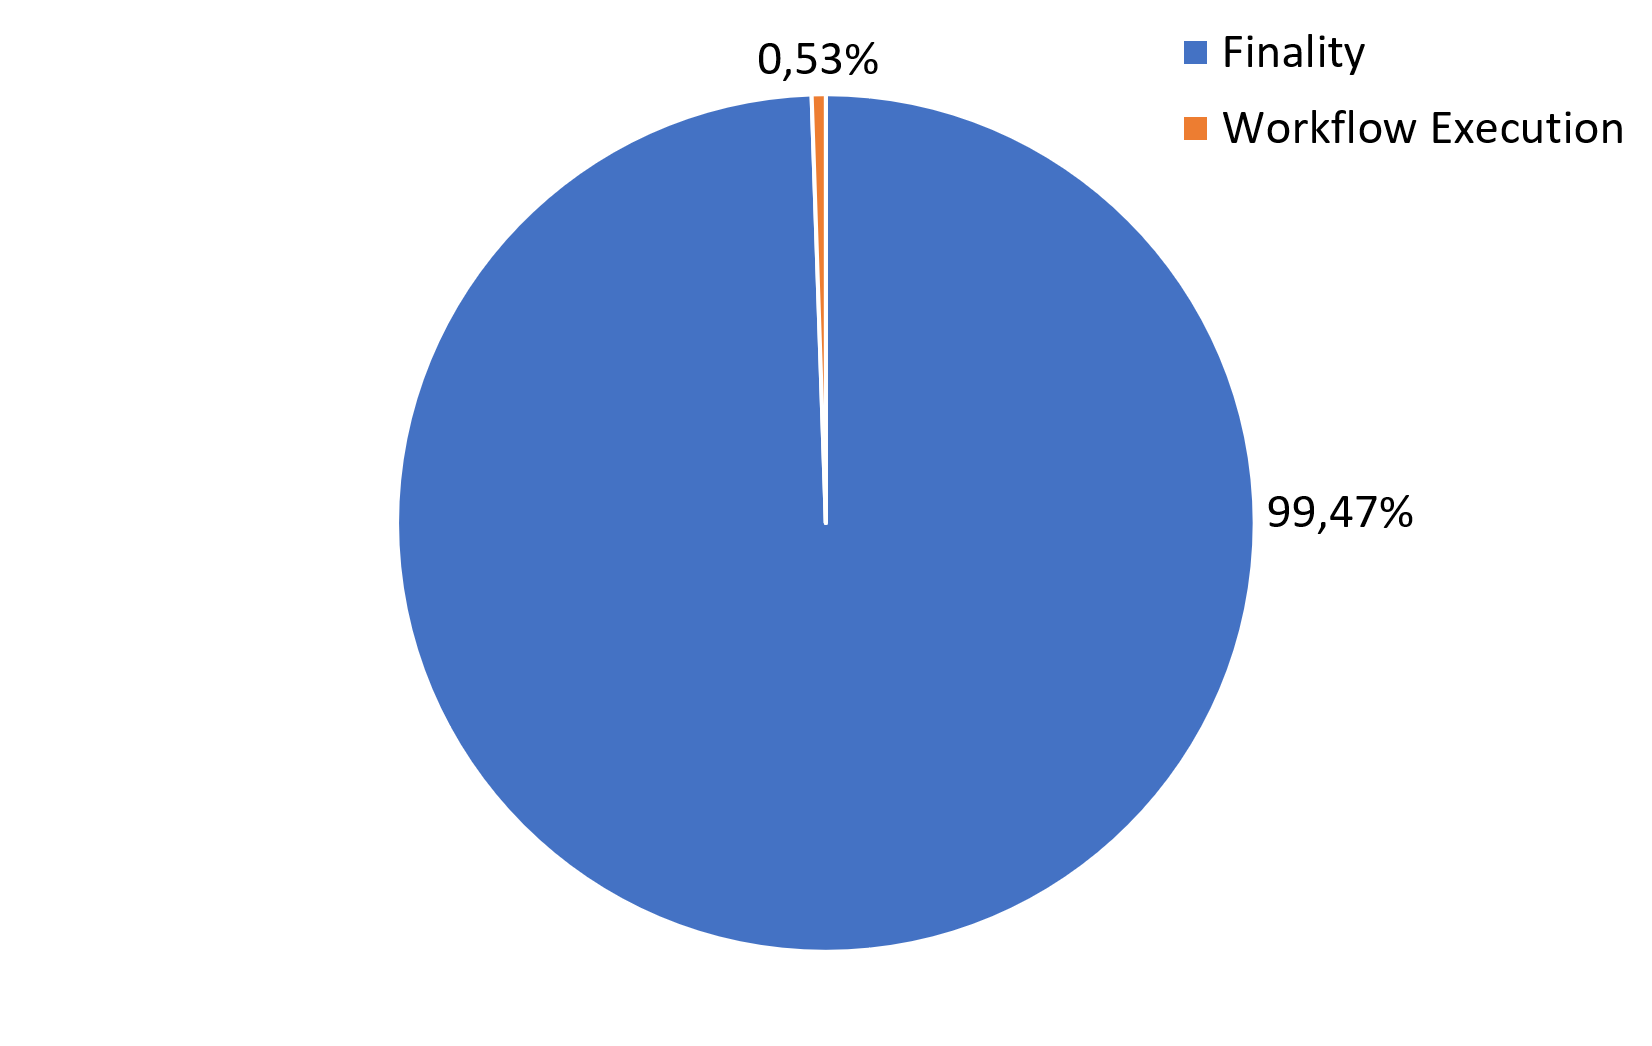
\includegraphics[width=.75\textwidth]{evaluation/graphics/experimental-analysis/finality-portion-pie-chart.png}}
    \caption{Pie chart illustrating a significant increase in workflow execution duration due to enforced transaction inclusion on the blockchain.}
    \label{fig:evaluation:simulations:pie_chart_transaction_inclusion_portion}
\end{figure}

Relying on enforced transaction inclusion has a significant impact on practical usability. Therefore, it should primarily be used for moderately to slow-paced workflows (requiring no more than 2 to 3 state transitions per minute). On the other hand, optimistic execution should only be used for very fast-paced workflows (more than four state transitions per minute), where little to no conflicts are expected. Fast-paced workflows that do produce conflicts between participants (due to conflicting rules being employed on each side, for example) must expect frequent rollbacks, which halts execution for a brief moment. Another scenario applicable for optimistic execution are tasks that only involve one participant because no two parties can disagree on a new workflow state\footnote{This also includes workflows only consisting of single party tasks (i.e.,\ entirely private workflows).}.

Nonetheless, it must be noted that these observations are only applicable when relying on an Ethereum-based consistency strategy. Optimistic execution might not even be considered viable when employing a strategy that, for example, leverages on a layer-2 rollup because the transaction inclusion duration is short enough to be neglected in the first place. Compared to existing approaches, a \gls{ttsm} with an \gls{evm}-based strategy typically performs between 20\%~\cite{untrusted_bp_execution_using_blockchain} and 25-times~\cite{runtime_verification_for_bp_utilizing_bitcoin} better regarding execution duration.

\subsubsection{Execution Cost}
\label{sec:evaluation:simulations:execution_cost}
Unlike execution duration, execution cost is tightly coupled with the number of participants involved in a certain operation, as discussed in the static analysis in section~\ref{sec:evaluation:static_analysis:blockchain_transactions}. Even though the cost of creating a workflow definition, an instantiation of such, and performing state transitions is linear in growth, deploying the required smart contract that stores the hashes of these operations remains constant. The evaluation for execution cost was conducted according to the methodologies used by Weber et al.~\cite{untrusted_bp_execution_using_blockchain,optimized_execution_of_bp_using_petri_nets_on_blockchain}, López-Pintado et al.~\cite{interpreted_bp_on_blockchain_weber}, Sturm et al.~\cite{lean_architecture_for_blockchain_based_process_execution}, Loukil et al.~\cite{interpreted_bp_on_blockchain_loukil}.

Table~\ref{tab:evaluation:simulations:gas_cost} shows the gas cost of each operation for each of the three scenarios. Given that the supply chain and incident management scenarios have the same number of participants but a different number of tasks (see table~\ref{tab:evaluation:simulations:structural_comparison}), one clearly identifies a strong correlation. The increasing costs come from the two-step process that each operation has to go through: (1) proposing a new definition, instantiation, or state transition, and (2) requiring all participants to send an accept or reject message.

\begin{table}[h]
\centering
\begin{tabular}{|l|c|}
    \hline
    & \multicolumn{1}{c|}{\bfseries Facility Management} \\ \cline{2-2}
    & Op.\ gas cost \\
    \hline
    Smart Contract         & 95,337 \\
    Workflow Definition    & 68,502 \\
    Workflow Instantiation & 68,502 \\
    State Transition       & 68,502 \\
    \hline
    & \multicolumn{1}{c|}{\bfseries Supply Chain} \\ \cline{2-2}
    & Op.\ gas cost \\
    \hline
    Smart Contract         & 95,337  \\
    Workflow Definition    & 137,004 \\
    Workflow Instantiation & 137,004 \\
    State Transition       & 137,004 \\
    \hline
    & \multicolumn{1}{c|}{\bfseries Incident Management} \\ \cline{2-2}
    & Op.\ gas cost \\
    \hline
    Smart Contract         & 95,337  \\
    Workflow Definition    & 137,004 \\
    Workflow Instantiation & 137,004 \\
    State Transition       & 137,004 \\
    \hline
\end{tabular}
\caption{Total gas cost of each operation type per scenario}
\label{tab:evaluation:simulations:gas_cost}
\end{table}

Even though the cost for a single blockchain transaction is rather small, with 22,834 gas, scenarios involving a lot of participants may be at a disadvantage. Nonetheless, the \gls{ttsm} prototype still performs better cost-wise than most other interpreted~\cite{interpreted_bp_on_blockchain_loukil,interpreted_bp_on_blockchain_weber}, and far better than most compiled approaches~\cite{untrusted_bp_execution_using_blockchain,optimized_execution_of_bp_using_petri_nets_on_blockchain} considering the three scenarios described above. Table~\ref{tab:evaluation:simulations:gas_cost_total} summarizes the total execution cost of each scenario, including smart contract deployment (even though only required once), workflow definition, instantiation, and all state transitions where each state transition is dispatched to every participant.

\begin{table}[h]
\centering
\begin{tabular}{|l|r|}
    \hline
    \textbf{Scenario} & \textbf{Total gas cost} \\
    \hline
    Facility Management & 574,851 \\
    Supply Chain        & 1,739,385 \\
    Incident Management & 1,602,381 \\
    \hline
\end{tabular}
\caption{Total gas cost of each scenario}
\label{tab:evaluation:simulations:gas_cost_total}
\end{table}

Notice that the total cost is still relatively high even though smart contract deployment is much more cost-efficient compared to existing approaches~\cite{interpreted_bp_on_blockchain_loukil,interpreted_bp_on_blockchain_weber}. This gives an opportunity for future work to improve the concept of a \gls{ttsm} by decoupling the execution cost from the number of involved participants. In particular, two areas for further research have been identified:

\begin{itemize}
    \item Investigation of applicable techniques to reduce the number of participants involved in an operation to a minimum\footnote{Only the middleman and the carrier have to accept or reject a state transition if supplier, manufacturer, and buyer are not involved in this process step, for example.}.
    \item Investigation of applicable blockchain-oriented software design patterns that allow decoupling of execution cost and the number of participants.
\end{itemize}

The first research challenge might require an in-depth analysis of statecharts and concepts such as the one proposed by Nakamura et al.~\cite{inter_organizational_bps_managed_by_blockchain}, where the interaction between participants is split into multiple statecharts. An interesting approach for the latter one, on the other hand, might be the off-chain signatures design pattern where all involved participants sign a proposed operation before writing the hash of the operation itself and the signatures to the blockchain~\cite{eberhardt17off_block,weber2019_architecture_for_dapps_blockchain_patterns}. Others, such as Carminati et al.~\cite{blockchain_for_secure_io_bp}, or Sun et al.~\cite{sun2021_survey_of_zkp_on_blockchain} motivate the usage of \glspl{zkp}, homomorphic encryption, or \glspl{tee} for concepts similar to a \gls{ttsm} in order to improve privacy and confidentiality and, regarding the challenges mentioned above, to reduce execution cost. Nonetheless, the proposed concept and the \gls{ttsm} prototype have shown their viability for use in real-world scenarios by demonstrating a rather low overall execution cost and exhibiting the potential for future improvements.

\subsubsection{Practical Conflict Resolution}
\label{sec:evaluation:simulations:conflict_resolution}
Scenarios such as the supply chain example described in section~\ref{sec:evaluation:simulations:descriptions:sc} are typically prone to create conflicts between participants. Resolving these, however, is rather trivial when properly employing a \gls{ttsm} due to its consistency, persistence, and verifiability properties. To demonstrate this, a conflict was simulated for the supply chain scenario, where a deadline was not met. It was successfully resolved by leveraging the time-travelling capabilities of the proposed concept and the prototype. By going back in time, the exact moment when delays were introduced was identified by the corresponding blockchain commitment reference. The hashes stored on-chain were then compared to the hashes of the operations stored off-chain. Therefore, the conflict was resolved by determining who introduced the delays by utilizing the auditability property of the blockchain.

\subsubsection{Privacy and Flexibility}
\label{sec:evaluation:simulations:privacy_flexbility}
Privacy was demonstrated thoroughly throughout the simulation of all three scenarios. All data is stored in hashed form on the blockchain when using the \gls{evm}-strategy. Therefore, even on public blockchains, only participants involved in the workflow can read and verify workflow-specific data. Leveraging on the concept's flexibility, future work may replace the \gls{evm}-strategy with a strategy based on \glspl{zkp}, layer-2 rollups, or homomorphic encryption, for example. Strategies like these hold potential regarding sharing and proving specific properties fulfilled by private workflow tasks without exposing confidential information~\cite{blockchain_for_secure_io_bp,sun2021_survey_of_zkp_on_blockchain}. Especially rollups, where many try to establish \gls{evm} compatibility, would enable the portability of the proposed approach and the smart contract presented in code listing~\ref{lst:evaluation:simulations:hash_storage}. Throughout the prototype implementation and evaluation, different strategies were employed to demonstrate the consistency module's flexibility. Nonetheless, metadata, such as hashes or \glspl{zkp}, still end up on the blockchain. Solving this issue is a topic for future research, especially regarding GDPR compliance.

% FOR REFERENCE
%\cite{untrusted_bp_execution_using_blockchain} & - & 334,646 & -\\
%\cite{optimized_execution_of_bp_using_petri_nets_on_blockchain} & - & 322,154 & -\\
%\cite{interpreted_bp_on_blockchain_weber} & 3,365,098 & 721,049 & \\
%\cite{lean_architecture_for_blockchain_based_process_execution} & - & 1,036,085\\
%\cite{interpreted_bp_on_blockchain_loukil} & 3,643,898 & 995,754\\


% \begin{itemize}
    % \item Use the facility maintenance use case to show that even a prototype of a \gls{ttsm} can handle real world business processes.
    % \item Experimental analysis using EVM because its portable
    % \item Solidity-ByteCode converter for layer-2 rollups
    % \item Is waiting for finality (i.e. latency) really practical? see \cite{untrusted_bp_execution_using_blockchain}
    % \item What about the cost? see \cite{untrusted_bp_execution_using_blockchain}
    % \item Only easy scenarios with prototype for evaluation. (Maybe use use cases from \cite{untrusted_bp_execution_using_blockchain})
    % \item Gas cost in paper \cite{interpreted_bp_on_blockchain_weber}
    % \item off-chain signature pattern might improve this even further!\cite{eberhardt17off_block,weber2019_architecture_for_dapps_blockchain_patterns}
    % \item Metrics might be: Execution cost, latency
    % \item SHOULD demonstrate real-world utility
% \end{itemize}



\section{Integration with Camunda's Zeebe}
\label{sec:evaluation:integration}
An aspect unneglectable in Design Science research is showing real-world utility of the produced artifacts~\cite{hevner2004_design_science}. One facet not discussed in this context until now is the integration of a \gls{ttsm} into an existing and well-established \gls{bpm} system to improve practical acceptance\footnote{Exchanging an existing solution with a new one is often times more complex and time consuming than integrating one into the other.}. Therefore, this section briefly introduces a possible adaptation of the existing \gls{ttsm} prototype in order to integrate it with Camunda's\footnote{\href{https://camunda.com/}{Camunda Website} (accessed on 2022-10-29)} workflow execution engine Zeebe\footnote{\href{https://docs.camunda.io/docs/components/zeebe/zeebe-overview/}{Camunda Docs: Zeebe} (accessed on 2022-10-29)}, to then discuss further opportunities. Camunda cloud\footnote{\href{https://console.cloud.camunda.io/}{Camunda Cloud Console} (accessed on 2022-10-29)} was used to provide access to instances of Camunda and Zeebe.


\subsection{Prototype Adaptations}
\label{sec:evaluation:integration:adaptations}
An integration requires some minor adaptations in the form of extensions to the prototype. The \textit{open-closed principle}, that the proposed concept for a \gls{ttsm} strictly follows, together with the modular design and the established event bus system, make it straightforward to create and attach new subsystems~\cite{meyer97_oo_software_construction,martin96_open_closed_principle,geirhos2015_design_patterns}. A new module called \textit{IntegrationsModule} has been added, to enable participants to dynamically integrate workflows and workflow instances into existing \gls{bpm} systems. It determines during runtime and, based on a given configuration which integrations to use. Furthermore, it also exposes the new \textit{ZeebeModule}. The \textit{ZeebeModule} is solely commissioned with the interaction between the \gls{ttsm} prototype and Camunda's Zeebe workflow execution engine. It stores its local data in the form of event logs as part of the global event bus and accesses it by aggregation by using projections\footnote{This is similar to the behavior of the rules module, for example.}. For the interaction between the prototype and Zeebe, the \textit{ZeebeModule} relies on the \textbf{zeebe-node 8.1.2}\footnote{\url{https://npmjs.com/package/zeebe-node} (accessed on 2022-11-29)} NodeJS library which allows the implementation of hooks that are triggered by Zeebe using gRPC\@. The code that links a \gls{ttsm} workflow instance with a Zeebe process instance is shown in listing~\ref{lst:evaluation:integration:zeebe_job_worker}.\\

\begin{lstlisting}[language=JavaScript,caption=Implementation of dynamic Zeebe job worker registration,captionpos=b,label=lst:evaluation:integration:zeebe_job_worker]
async linkProcessInstance(instance: WorkflowInstanceProposal) {

  // Job worker function to advance TTSM workflows.
  const handler: ZBWorkerTaskHandler = (job: ZeebeJob) => {
    try {
      this.workflowService.advanceWorkflowInstance(
        instance.id,
        {
          event: job.type,
          payload: job.variables
        }
      );
    } catch (error) {
      return job.fail(error.message);
    }
    return job.complete();
  };

  // Each workflow has a list of state names (strings).
  for (const nextStateName of instance.workflow.states) {

    // Register a job worker for each consistency task.
    this.zeebeClient.createWorker({
      taskType: nextStateName,
      taskHandler: handler
    });
  }
}
\end{lstlisting}

The \textit{ZeebeModule} creates a new worker for each state in the given workflow. Whenever a participant advances the state inside Camunda, the corresponding worker is triggered and either returns a \textit{fail} or \textit{complete} response to Zeebe. Note that this is only a basic prototypical implementation of such an integration that should serve as proof of concept. It is not part of the actual \gls{ttsm} concept itself. In a full-fledged implementation, the \textit{ZeebeModule} should await inclusion of the transaction into a block on the blockchain before returning a response and notify all participants to keep the workflow state synchronized. The adaptations described above are also available on GitHub\footnote{\url{https://github.com/danielkleebinder/ttsm-prototype} (accessed on 2022-11-29)}.

% \begin{itemize}
    % \item New module ``ZeebeModule'' that stores its local data in the event store and projection aggregates data.
    % \item Workflow definitions are deployed on Zeebe every time a \textbf{\textit{Consistency.Workflow.Received}} internal persistence event is detected.
    % \item Workflow instances are deployed on Zeebe every time a \textbf{\textit{Consistency.Instance.Received}} internal persistence event is detected.
    % \item Zeebe client for NodeJS has been used.
    % \item Zeebe connection might be integrated into workflow instantiation
    % \item Very basic prototypical implementation. The ``ZeebeModule'' should probably only complete a job if it has a commitment reference on the blockchain and all participants are aware of the state transition.
    % \item This implementation is only a proof of concept!!! And not part of the actual \gls{ttsm} concept.
% \end{itemize}

\subsection{Workflow Execution}
\label{sec:evaluation:integration:execution}
In order to leverage on the properties of a \gls{ttsm}, the \gls{bpmn} diagrams used in Camunda must follow a certain format. Each task in Camunda that wants to interact with the \gls{ttsm} must be defined as a ``service task'' to trigger a job worker. These are tasks dedicated to ensure consistency and traceability using a \gls{ttsm} and mark the interfaces between participants. An example of such a \gls{bpmn} diagram is given in figure~\ref{fig:evaluation:integration:service_tasks}.

\begin{figure}[h]
    \makebox[\textwidth][c]{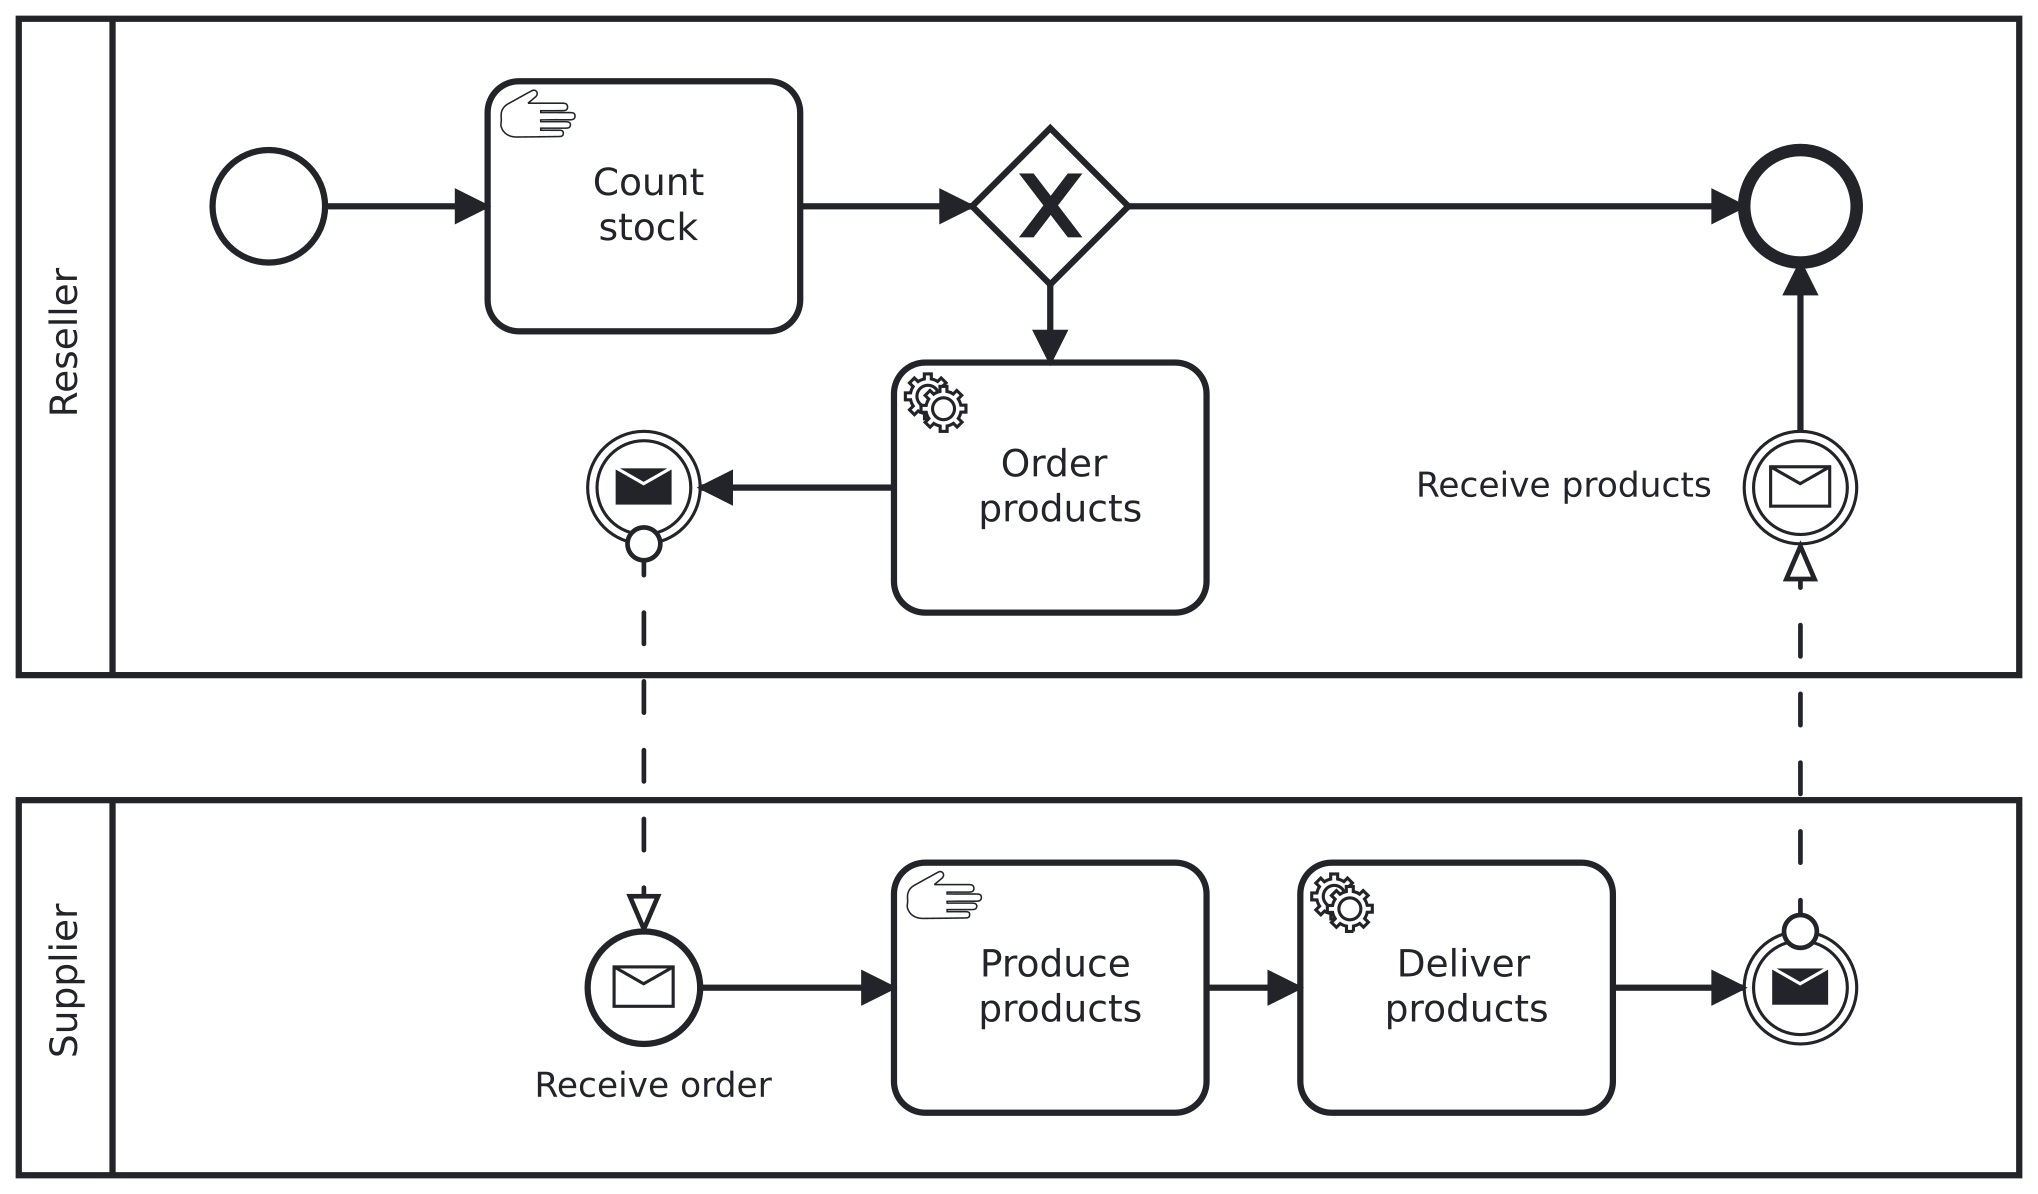
\includegraphics[width=.7\textwidth]{evaluation/graphics/integration/camunda-supplier-reseller.png}}
    \caption{Exemplary reseller-supplier scenario with service tasks before each interaction.}
    \label{fig:evaluation:integration:service_tasks}
\end{figure}

A reseller counts her stock and, depending on the result, orders products from the supplier. The ``Order products'' activity is a service task that triggers a \gls{ttsm} job worker, which handles the consistency concerns and the interaction between participants. After the supplier received the order and produced all required products, the deliver products service task is invoked, eventually leading to product delivery and completing the workflow. For the \gls{ttsm} to properly interact with Camunda and Zeebe, a choreography diagram solely concerned with the interactions between participants must be derived. Such an integration-compliant diagram only contains the service tasks and the names of the participants. Other activities are treated as private. A dedicated consistency service task must be specified if private activities require consistency. This means that service tasks that trigger a job worker in a \gls{ttsm} are not limited to interactions between two or more participants; however, they are predestined for it. Private service tasks require choreography activities to specify the same party as initiator and receiver. Figure~\ref{fig:evaluation:integration:service_tasks_choreography} shows the choreography diagram of the reseller-supplier scenario from figure~\ref{fig:evaluation:integration:service_tasks} above.

\begin{figure}[h]
    \makebox[\textwidth][c]{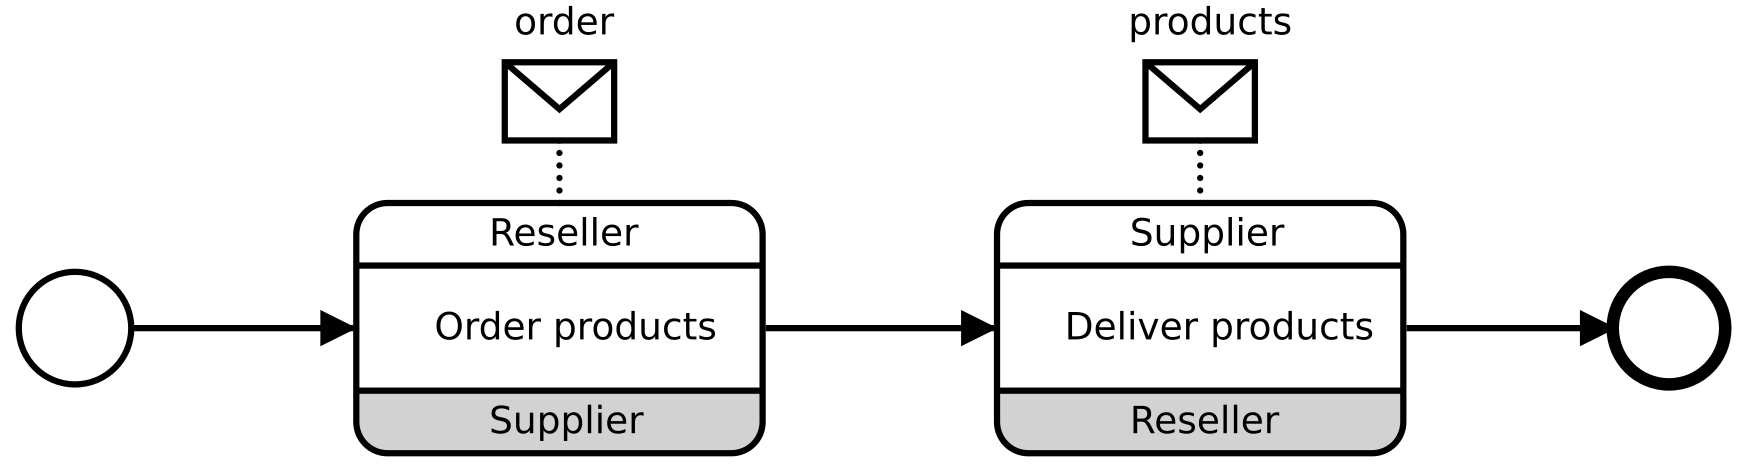
\includegraphics[width=.7\textwidth]{evaluation/graphics/integration/camunda-supplier-reseller-choreography.png}}
    \caption{Choreography of the reseller-supplier scenario.}
    \label{fig:evaluation:integration:service_tasks_choreography}
\end{figure}

This choreography diagram is then converted to statecharts and deployed by the \gls{ttsm}. Even though the deployment and instantiation are directly executed on the \gls{ttsm}, the workflow instance execution is performed using the graphical UI of Camunda. All necessary configuration of the Zeebe-integration is part of the deployment and the instantiation of the workflow.

% \begin{itemize}
    % \item Each task in Camunda that wants to interact with the \gls{ttsm} must be defined as ``service task'' to allow a job worker to be triggered. Dedicated tasks for consistency so to say.
    % \item Deployment and instantiation of a workflow must be executed by the \gls{ttsm}, state transitions are then performed by Zeebe inside Camunda.
    % \item Requires converter from statecharts to Zeebe-compliant \gls{bpmn} diagrams (hard-coded at the moment).
    % \item State transitions must be defined as Zeebe task definitions as an extension to standard \gls{bpmn}.
% \end{itemize}

\subsection{Summary and Discussion}
\label{sec:evaluation:integration:summary}
The evaluation performed in this section has introduced some minor extensions to the \gls{ttsm} prototype by adding a \textit{ZeebeModule} for integration into Camunda's Zeebe workflow execution engine. It allows participants to execute workflow instances using the graphical UI of Camunda while keeping auditability, traceability, and consistency properties of a \gls{ttsm}. However, the integration of workflow deployment was not possible. The evaluation of Camunda connectors\footnote{\href{https://docs.camunda.io/docs/components/integration-framework/connectors/use-connectors/}{Camunda Docs: Connectors} (accessed on 2022-10-29)} and Zeebe job workers\footnote{\href{https://docs.camunda.io/docs/components/concepts/job-workers/}{Camunda Docs: Job Workers} (accessed on 2022-10-29)} shows that they are no suitable solutions, because they are not concerned with the entirety of the workflow, but only with single tasks. This yields the following research challenge for future work:

\begin{itemize}
    \item Investigation of integration strategies that allow participants to deploy and instantiate new workflows using Camunda and its underlying workflow execution engine Zeebe instead of relying on the \gls{ttsm}.
\end{itemize}

Answering this research challenge might include writing a custom Camunda plugin\footnote{\href{https://docs.camunda.org/how-tos/cockpit/develop-a-plugin/}{Camunda Docs: Custom Plugins} (accessed on 2022-10-29)}. Nonetheless, the integration seems to hold great potential. Therefore, a more in-depth investigation considering the integration of a \gls{ttsm} into Camunda and Zeebe is advised as part of future work. This might include replacing parts of the Zeebe or Camunda architectures with concepts proposed in this work or vice versa by replacing the workflow module with Zeebe, for example. Even though the integration evaluation in this work has only been a proof of concept with very little functionality, it demonstrated interesting prospects that future work could leverage on.

% \begin{itemize}
    % \item A more in-depth investigation is advised considering \gls{ttsm}-integration into Camunda and Zeebe.
    % \item Integration seems to hold great potential
    % \item Workflow module can be replaced with Zeebe, for example
% \end{itemize}

\subsection{Research Question 3}
\label{sec:evaluation:integration:rq3}
To answer the third research question:

\begin{quote}
    \emph{Which aspects must be adapted to close the gap between the state of the art and a privacy-preserving \gls{bct}-based state machine that allows time-travel verification?}
\end{quote}

Existing workflow execution systems already hold great potential when it comes to the integration of the concept for a \gls{ttsm}. Not only is this a viable option when auditability or traceability are required, but the expenditure for such a venture also seems to be relatively low. Concepts proposed in related work that leverage on blockchains, however, have shown a formidable lack of flexibility and privacy. This can be traced back to the fact that almost all concepts rely on running code directly on layer-1 blockchains. Even though some concepts aim to circumnavigate or even solve the shortcomings imposed by layer-1 blockchains, neither can mitigate the majority of them. To close the gap between the state of the art and a privacy-preserving \gls{bct}–based state machine that allows time-travel verification, future concepts might want to start building on layer-2 or even start targeting layer-2 rollups and build on layer-3 instead of directly leveraging on blockchains. Using the blockchain as a supportive third-party system that provides certain properties increases the flexibility of the system built on top of it and reduces its cost. Nonetheless, the potential imposed by a \gls{bct}–based state machine that only takes advantage of blockchain properties without directly building, and thus constraining itself by it, is not to be neglected.

% This, however, might require future work to identify desirable layer-1 properties, which properties layer-2 or layer-3 applications must fulfill, and which layer-1 properties can be transferred to layer-2 or layer-3 without canceling out desirable properties from underlying layers.


% \begin{itemize}
    % \item Do not use layer-1 blockchains, build on layer-2 or even better on layer 3.
% \end{itemize}
